\documentclass[12pt]{article}
\usepackage[a4paper, margin=2.5cm]{geometry} % layout
\usepackage{parskip} % line breaks between paragraphs
\usepackage{float} % control over position of figures, tables
\usepackage{hyperref} % references, citations
\usepackage{graphicx} % plots
\usepackage{amsmath, amsfonts} % advanced maths
\usepackage{algorithm, algpseudocode} % pseudocode
\title{Learning Distributions with Neural Networks}
\author{}
\date{\today}
\begin{document}
\maketitle

\section{Abstract}

\section{Introduction}

\section{Frequentist vs Bayesian Neural Networks}
\label{sec_nn_vs_bnn}

Neural networks are most commonly used for prediction: namely regression or classification. In this setting, they map input predictors $x$ to the output variable $y$. So we can think of a neural network simply as a function that maps $x \rightarrow y$, \textit{conditioned} on some specific parameters of the neural network. In probability jargon, the neural network is a likelihood function, $p(y | x, \theta)$.

Let's assume we observe some new predictors $\tilde{x}$ and we want to predict the response variable $\tilde{y}$. For example, an autonomous vehicle observes a new object and needs to classify it, or it observes a pedestrian and needs to predict her movement. In this context, we are interested in the quantity $p(\tilde{y} | \tilde{x})$, but a neural network only gives us $p(\tilde{y} | \tilde{x}, \theta)$. The solution to this problem is to \textit{train} the neural network on some observed data $(x, y)$ by learning the distribution $p(\theta | x, y)$ and then marginalize over this distribution during prediction, obtaining the distribution $p(\tilde{y} | \tilde{x}, x, y)$:

\begin{equation}
p(\tilde{y} | \tilde{x}, x, y) = \int_{-\infty}^\infty p(\tilde{y}, \theta | \tilde{x}, x, y) d\theta =   \int_{-\infty}^\infty p(\tilde{y} | \tilde{x}, \theta) p(\theta | x, y) d\theta
\label{eq_post_pred}
\end{equation}

There are two distinct approaches to learning $p(\theta | x, y)$, based on \textit{frequentist} and \textit{Bayesian} principles. In the frequentist context, we will estimate the value of $\theta$ and assume that the true value of $\theta$ is equal to the estimated value with $100\%$ probability. Clearly, this is a naive assumption and no one actually believes this, but it is an assumption that we have to make in order to marginalize over $\theta$. Perhaps we might avoid claiming that we know the true value of $\theta$ with certainty, but then we cannot marginalize over $\theta$, i.e. we cannot really make any predictions of the form $p(\tilde{y} | \tilde{x}, x, y)$. Since our goal is to obtain predictions, we will assume that frequentist inference is equivalent to assuming that we know the true value of $\theta$ with certainty, i.e. we will assume a Dirac delta distribution over $\theta$.

In contrast, in Bayesian inference, we must assume some prior distribution over $\theta$, before observing any data and then update this belief given the observed data $(x, y)$. This is achieved using Bayes' rule:

\begin{align}
\begin{split}
p(\theta,y|x) &= p(\theta,y|x) \\
p(\theta|x,y)p(y|x) &= p(y|x,\theta)p(\theta|x)\\
p(\theta|x,y) &= \frac{p(y|x,\theta)p(\theta|x)}{p(y|x)}\\
p(\theta|x,y) &= \frac{p(y|x,\theta)p(\theta)}{\int_{-\infty}^\infty p(\theta, y|x) d\theta}\\
p(\theta|x,y) &= \frac{p(y|x,\theta)p(\theta)}{\int_{-\infty}^\infty p(y|x,\theta)p(\theta) d\theta}\\
p(\theta|x,y) &\propto p(y|x,\theta)p(\theta)
\end{split}
\label{eq_posterior}
\end{align}

In Bayesian inference, the choice of the prior distribution over $\theta$ is subjective, since we must make this choice \textit{before} observing any data. The resulting posterior distribution is typically very complex and has no closed-form solution. Instead, it must be numerically approximated -- this is discussed later.

\section{Neural network}

A neural network can act as a universal function approximator. Hence, we can train a neural network do fit our observed data. For example, we can design a neural network that will output a single number, which will represent the point estimate for a given observation. Alternatively, we can assume that the observed value $y$, conditional on the predictors $x$, will be distributed according to a distribution belonging to a given family (e.g. Normal). Then, given a set of predictors, the network can output a vector corresponding to the parameters of the given distribution. In other words, the network's output will be a distribution over $y$, rather than a single point estimate. 

\subsection{Multilayer perceptron}

The multilayer perceptron (MLP) is arguably the simplest neural network architecture. We can think of it as a series of layers, where each layer performs a non-linear transformation. These layers are sequentially chained, so that the output of one layer is the input to the next layer.

Let's denote the input to the MLP as $x_1$ (this is a vector of predictors for a single observation in a dataset). This input will be passed to the first layer, which will perform a non-linear transformation of $x_1$ and return a transformed output, denoted $x_2$. Next, $x_2$ will be passed to the second layer, which will transform it and output $x_3$. This process will be repeated until we reach $x_n$, the output layer. So we can think of the MLP as the following series of transformations, where each arrow corresponds to one layer of the network:

\begin{equation}
x_1 \rightarrow x_2 \rightarrow x_3 \rightarrow \ldots x_{n_1} \rightarrow x_n
\end{equation}

The layer $x_1$ is called the \textit{input layer}, $x_n$ is called the \textit{output layer}, and all the layers in between are called \textit{hidden layers}. Each of the layers consists of a single matrix multiplication and a nonlinearity:

\begin{equation}
x_i = \sigma(W_i x_{i-1} + b_i)
\end{equation}

Essentially, the input to the layer $x_i$ is multiplied by a matrix $W_i$, shifted by a \textit{bias} vector $b_i$, and transformed through a nonlinear function denoted $\sigma$. The layers are called \textit{fully-connected} since each component of the input $x_{i-1}^j$ is connected to each component of the output $x_i^k$ through some matrix weight $W_{jk}$.

Another way to visualize the MLP is as a graph of connected nodes that represent \textit{artificial neurons} (Fig. \ref{fig_mlp}). In every layer, every node is connected to every node in the previous layer and every node in the following layer (hence the name \textit{fully-connected}). We can think of the connections between the neurons as the matrix parameters $W_{jk}$, corresponding to the strength of each connection. At a very high level, this architecture is inspired by the human brain, although it has to be noted that the analogy is loose.

\begin{figure}[ht]
\centering
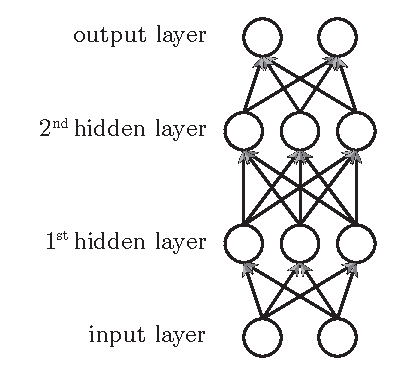
\includegraphics[width=6cm]{illustrations/mlp.pdf}
\caption{}
\label{fig_mlp}
\end{figure}

The role of the nonlinearity $\sigma$ (also called an \textit{activation function}) is essential. If there was no nonlinearity in the network, each layer would only perform some specific linear transformation. However, the composition of linear transformations is still just a linear transformation. So without the nonlinearity, increasing the network's number of layers would have essentially no effect. In contrast, \textit{with} the nonlinearity, the more layers are used, the more complex a function the neural network can express. Historically, it was common to apply the \textit{sigmoid} activation function, which monotonically maps all real numbers to the interval $(-1, 1)$:

\begin{equation}
\sigma_{\textrm{sigmoid}}(x) = \frac{1}{1 + e^{-x}}
\end{equation}

While this is a perfectly reasonable activation function to use, in practice, the ReLU activation (\textit{rectified linear activation function}) seems to work just as well and it is easier to compute:

\begin{equation}
\sigma_{\textrm{ReLU}}(x) = \max(0, x)
\end{equation}

\subsection{Loss function}
\label{sec_loss_fn}

Neural networks are typically trained using gradient descent. The idea is to define a loss function to evaluate the discrepancy between the neural networks's desired output and its actual output, and then minimize this discrepancy (loss). A low value of the loss function implies that the output of the neural network is close to the desired output.

For example, when the neural network is designed to output point estimates, we can use the sum of squared residuals as the loss function: $\sum_i (\hat{y_i} - y_i)^2$. Conversely, when the neural network's output is a probability distribution, we can maximize the likelihood of the observed data: $\prod_i \hat{p}(y_i)$. However, often, the likelihood for a single observation is a very small number, much smaller than zero. Taking a product over thousands of very small numbers results in a number that is extremely small, easily smaller than $10^{-1000}$. When computers store numbers, they must do so with a fixed precision, so that the numbers can be encoded by a fixed number of bits. Typically, this is no higher than 64 bits, split up between the number's \textit{mantissa} (value) and \textit{exponent} (order of magnitude). Out of the 64 bits used to store the number, only 11 are used to store its exponent, meaning the smallest number that can be natively stored on modern computers is $2^{-2^{10}} = 2^{-1023} \approx 10^{-308}$. While this is a very small number, it is not small enough to store some likelihood values. As a result, any likelihood smaller than roughly $10^{-308}$ would get rounded down to zero. This an error that must be avoided, since it would prevent us from taking derivatives of the likelihood. Typically, this problem is avoided by working with the (negative) logarithm of likelihood ($\textrm{NLL}$), rather than the likelihood itself: $\textrm{NLL} = -\log(\prod_i \hat{p}) = -\sum_i \log\hat{p}(y_i)$.

\subsection{Gradient descent}

A neural network is defined by its architecture (e.g. number and type of layers) and its parameters, denoted $\theta$. Typically, the architecture is defined by a human and fixed for the duration of training. Training is achieved only by modifying the parameters of the neural network. The most common way to do this is to iteratively differentiate the loss function w.r.t. the parameters and then update the parameters in the direction of decreasing loss. This is called \textit{gradient descent}. More specifically, the parameters of the neural network at step $i+1$ are equal to the parameters at the previous step ($i$) plus a step in the direction of decreasing loss:

\begin{equation}
\theta_{i+1} \leftarrow \theta_{i} - \gamma \frac{\partial L}{\partial \theta_i}
\label{eq_sgd}
\end{equation}

In the above equation, $\gamma$ is called the \textit{learning rate} and it dictates how far along the direction of decreasing loss we move. The issue is that the gradient is only a linear approximation of the loss function, so stepping too far could cause the training procedure to become unstable. Conversely, setting the learning rate too small will increase the number of steps required to reach convergence, resulting in an unnecessary increase in computational cost.

In practice, modern machine learning libraries implement \textit{automatic differentiation}, meaning they can analytically differentiatiate any complex function that is composed of simpler differentiable functions. A neural network is technically just a function composed of thousands (or millions, possibly billions) of parameters and simple differentiable operations like addition and multiplication. So, in practice, it suffices to define a neural network architecture and let the library compute its derivates. However, for the sake of understanding, it can still be helpful to derive the derivative of loss w.r.t. parameters by hand. This helps provide intuition behind the inner workings of modern machine learning libraries.

Let's assume that we are using an MLP where each layer has only a single parameter. Then, we can apply the chain rule to expand the derivative of the loss function w.r.t. the neural network's parameters $W_i$:

\begin{equation}
\frac{\partial L}{\partial W_i} = \frac{\partial L}{\partial x_n} \frac{\partial x_{n-1}}{\partial x_{n-2}} \ldots \frac{\partial x_{i+2}}{\partial x_{i+1}} \frac{\partial x_{i+1}}{\partial W_i}
\end{equation}

Inside the above expression, there is a repeating term of the form $\frac{\partial x_{i}}{\partial x_{i-1}}$. In order to compute it, it is helpful to define $z_i := W_i x_{i-1} + b_i$. Then:

\begin{equation}
\frac{\partial x_{i}}{\partial x_{i-1}} = \frac{\partial \sigma(z_{i})}{\partial x_{i-1}} = \sigma'(z_i) \frac{\partial z_{i}}{\partial x_{i-1}} = \sigma'(W_i x_{i-1} + b_i) W_{i-1}
\end{equation}

A similar expression holds for the bias terms $b_i$:
\begin{equation}
\frac{\partial x_{i}}{\partial x_{i-1}} = \sigma'(W_i x_{i-1} + b_i)
\end{equation}

Then, if we know the derivative of the loss function $L$, we know the the derivatives of all the parameters of the network and we can iteratively apply gradient descent to train the network.

In reality, the parameters of each layer ale vectors, rather than scalars. Surprisingly, the same equations still hold. The only difference is that instead of computing scalar derivates, we need to compute the Jacobians of each transformation, which have the same form as the scalar expression. The chain rule also applies in a similar way, except that instead of multiplying scalars, we matrix-multiply the Jacobians of each transformation.

\subsection{Stochastic gradient descent}

When large neural networks are trained on large datasets (e.g. millions of images), it would be extremely expensive to evaluate each gradient update on the whole dataset. In order to speed up the training, the dataset is typically split-up into several smaller \textit{mini-batches}, and the gradient is computed independently on each of these mini-batches. This method is called \textit{stochastic gradient descent} (SGD).

The term \textit{epoch} is commonly used as a unit to measure how many dataset samples a neural network was trained on. One epoch means that the model saw each instance from the dataset exactly once. Two epochs means that the model saw the whole dataset twice... and so on. In full-batch gradient descent, one epoch corresponds just to a single update of the model parameters. In contrast, if the dataset is split into 100 mini-batches, one epoch represents 100 gradient updates. While each of these updates is noisy (it is only an approximation of the true gradient, based on the whole dataset), it turns out that many noisy gradient updates (i.e. SGD) typically results in faster training compared to full-batch gradient descent.

Another advantage of SGD is rooted in hardware. Neural networks are typically trained on hardware like graphics processing units (\textit{GPUs}) or tensor processing units (\textit{TPUs}). These devices are very fast at parallel computing, such as matrix multiplication and other element-wise operations. However, they also have limited memory available: typically in the range 8 -- 80 GB. During backpropagation, this is enough memory only for a few images, but in low-dimensional regression, it can actually be enough to store the whole dataset.

Within this essay, the terms \textit{gradient-descent} and \textit{SGD} are used interchangeably, even though full batches are always used. Since all experiments use a small dataset, using mini-batches is not necessary. However, if a larger dataset were used, using mini-batches would be preferable. For the purposes of this essay, there is no differnce between gradient descent and stochastic gradient descent. 

\subsection{Learning rate schedule}

In Eq. $\ref{eq_sgd}$, we see that the SGD update depends on the learning rate $\gamma$. But what is a good value of $\gamma$? When the learning rate is too large, $\theta$ may fail to converge; when the learning rate is too small, training will take too long. One common solution is to use use a \textit{learning rate schedule}, rather than a constant learning rate.

All experiments in this project use an \textit{exponentially decaying} learning rate. The idea is that in the early phase of training, we can get away with a high learning rate and achieve fast convergence, while as we approach a local minimum, the learning rate needs to be decreased such that we can carefully descent into that minimum. This is implemented by multiplying the learning rate after each update by a constant rate $r$ that is very slightly smaller than zero:

\begin{equation}
\gamma_{i+1} \leftarrow r \gamma_i
\end{equation}

\subsection{Loss landscape}
\label{sec_loss_landscape}

Whether a neural network is trained to maximize the log-likelihood (i.e. find the \textit{maximum likelihood / ML} solution) or the log-posterior (i.e. find the \textit{maximum a posteriori / MAP} solution), the geometry of its loss as a function of its parameters is interesting to study.

Let's assume we observe the data in Fig. \ref{fig_1d_dataset} and try to train a neural network to model the conditional distribution $p(y | x)$.

\begin{figure}[ht]
\centering
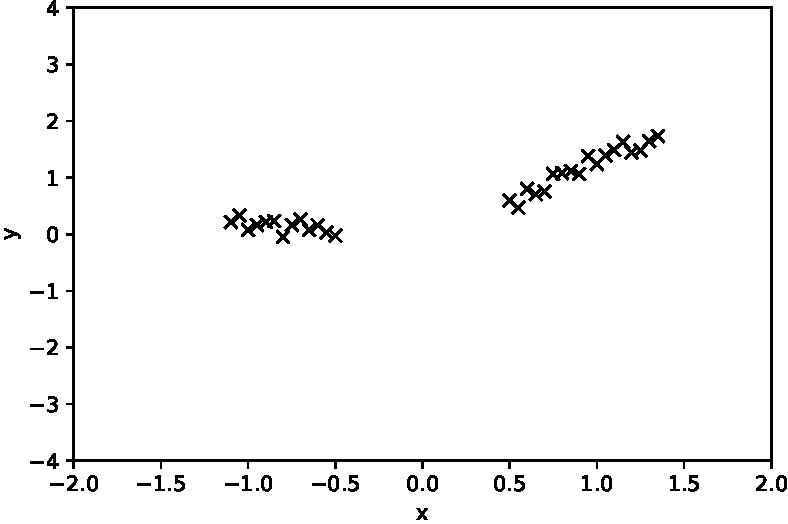
\includegraphics[width=9cm]{plots/1d_dataset.pdf}
\caption{}
\label{fig_1d_dataset}
\end{figure}

We use an MLP with a single hidden layers consisting of 50 nodes and a $N(0, 0.1^2)$ prior over $\theta$ . The network outputs the tuple $(\mu, \sigma^2)$ for each observation and we assume that $y \sim N(y, \sigma^2)$. We initialize six networks like this, each with parameters drawn independently from a $N(0, 0.22^2)$ distribution. Footnote: using a larger variance to initialize the networks would cause problems with numerical stability. Afterwards, we train each network using SGD until convergence. We set the loss function proportional to the logarithm of the posterior distribution. Fig. \ref{fig_1d_ens_predictions} shows the predictions of each of these networks:

\begin{figure}[ht]
\centering
\makebox[\textwidth][c]{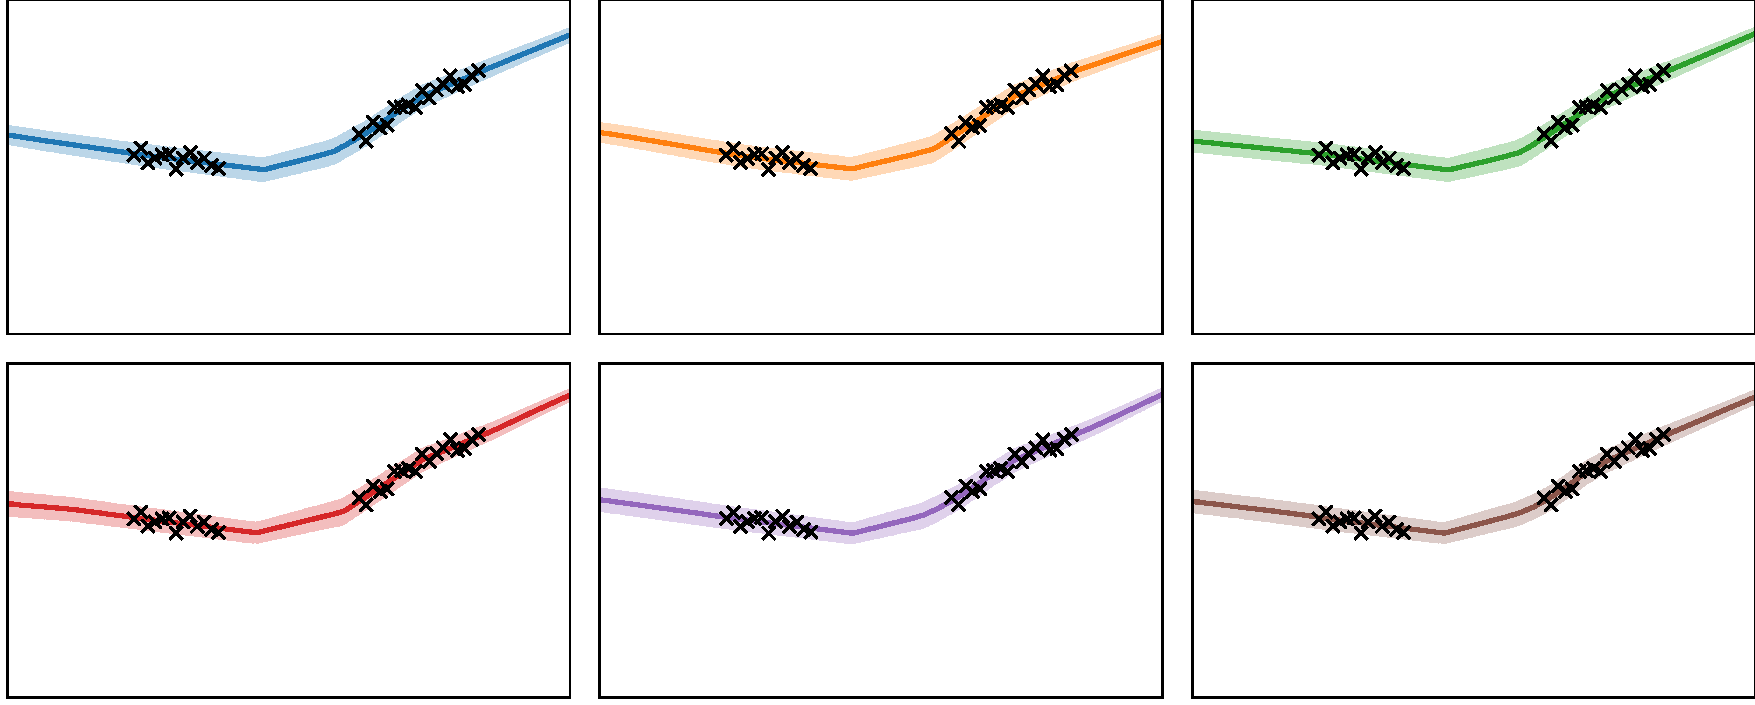
\includegraphics[width=18cm]{plots/1d_ens_predictions.pdf}}
\caption{}
\label{fig_1d_ens_predictions}
\end{figure}

It appears that each of these independent networks has learned the same function. However, the parameters of each network are different. This is evident from Fig. \ref{fig_1d_ens_param_distance}, which shows the $L_1$ distance between the parameters of the first network and the other five during training. At initialization, the $L_1$ norms of the parameters of each networks is between $0.18 - 0.25$ and they remain in this range after training. At initialization, the distances are all between $0.2 - 0.3$ and they only change very little during training. This implies that each of the 6 networks has converged to a different solution in the parameter space, since the distances are roughly constant and roughly equal to the norms of the parameters.

\begin{figure}[ht]
\centering
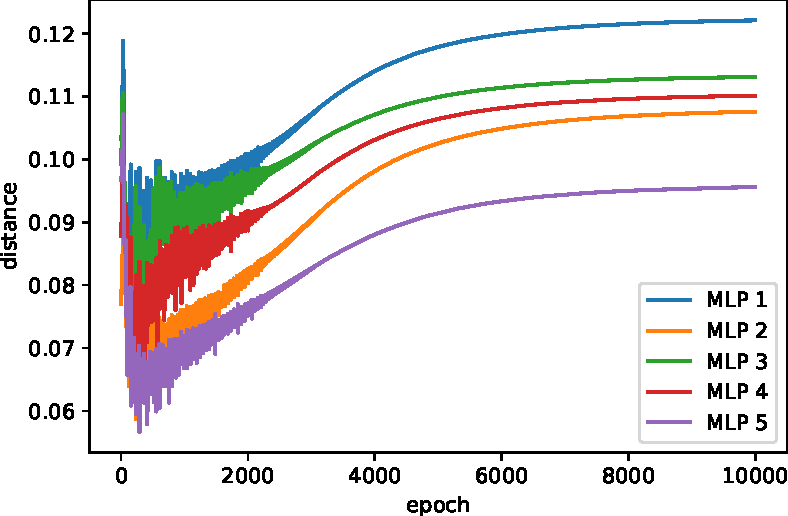
\includegraphics[width=9cm]{plots/1d_ens_param_distance.pdf}
\caption{}
\label{fig_1d_ens_param_distance}
\end{figure}

Part of the reason behind this is that modern neural networks are typically \textit{over-parametrized}, meaning there are many different sets of parameters $\theta$ that fit the observed data equally well. \cite{underspecification, deep_ens, mode_connectivity} Each of the networks in this example were initialized differently and SGD tends to converge to a solution that is close to the initialization. Hence, each of the different initializations resulted in a different SGD solution.

A natural question that arises is: \textit{what does the geometry of the loss function look like?} One way to peek at this high-dimensional landscape is to plot the plane described by three independent SGD solutions. Let's denote the parameters of these three networks $\theta_0, \theta_1, \theta_2$. Next, let's define a new coordinate system under which the coordinates of these solutions are $(-1, 0), (1, 0), (1, 0)$. This can be achieved by defining the following auxiliary variables:

\begin{align}
\begin{split}
\theta_m &= \frac{\theta_0 + \theta_1}{2} \\
d_x &= \theta_1 - \theta_m \\
d_y &= \theta_2 - \theta_m
\end{split}
\end{align}

Then, any point $R$ along the surface described by $\theta_0, \theta_1, \theta_2$ can be mapped to the $2D$-coordinates $(x, y)$ as follows:

\begin{equation}
R = \theta_m + x d_x + y d_y
\end{equation}

\begin{figure}[ht]
\centering
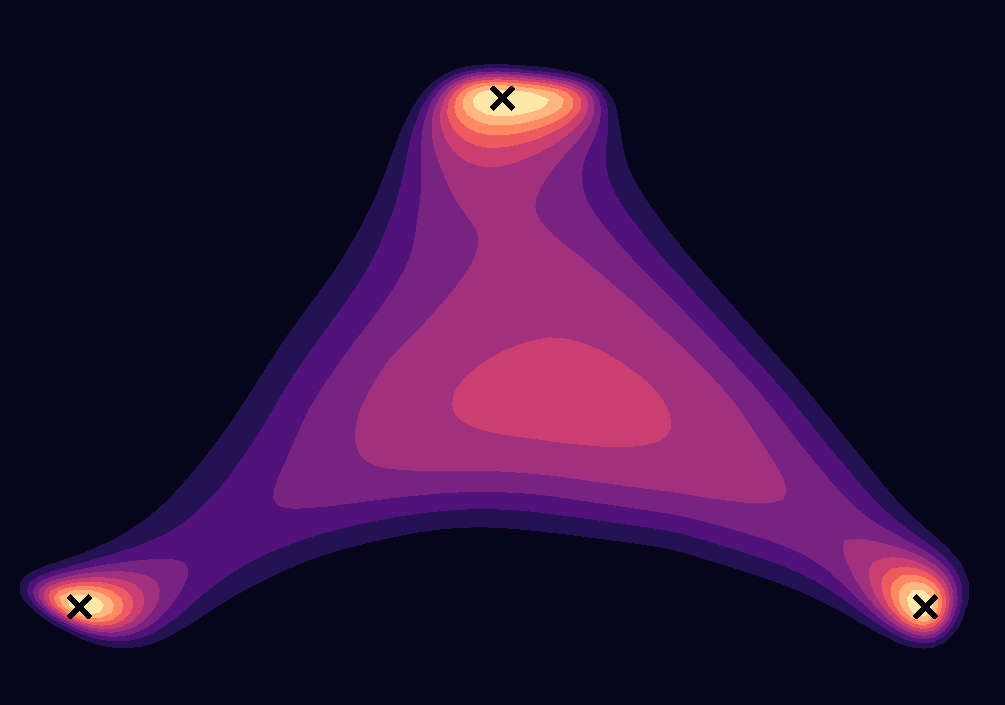
\includegraphics[width=14cm]{plots/loss_landscape.pdf}
\caption{A contour plot of the value of the loss function of a single-layer MLP. The three crosses connected by dashed grey lines represent three independent SGD solutions. They define the plane along which the loss is evaluated, displayed by the contours.}
\label{fig_loss_landscape}
\end{figure}

Fig. \ref{fig_loss_landscape} shows the plane described by the three solutions $\theta_0, \theta_1, \theta_2$. Notice that $\theta_1$ and $\theta_2$ (the middle and right solutions) appear to be connected by a low-loss region, while $\theta_0$ appears to be disconnected from the other two solutions.

In general, but especially in larger networks \cite{mode_connectivity}, a linear path between two SGD solutions will contain a region of very high loss, comparable to a randomly-initialized network. At the same time, deviating from an SGD solution in a random direction will also cause the loss to increase rapidly \cite{swag}. However, for any two SGD solutions, there is typically a low-loss tunnel connecting them. The loss along this tunnel is approximately equal to the two SGD solutions. \cite{mode_connectivity} Fig. \ref{fig_loss_landscape} hints at this phenomenon, although the loss does decrease slightly along the low-loss path from the middle solution to the right solution.

Garipov et al \cite{mode_connectivity} devise a simple method to find a low-loss tunnel between any two SGD solutions. Consider two arbitrary SGD solutions $\theta_0$ and $\theta_1$. Then, for any proposed path connecting $\theta_0$ and $\theta_1$, we will uniformly sample points from this path and evaluate the loss along this points. The goal is to find a path where the sum of these losses is the lowest. They obtained good results searching for a path $\theta_t$ defined by a quadratic Bézier curve:

\begin{equation}
\theta_t = (1-t)^2 \theta_0 + 2t(1-t) \theta^* + t^2 \theta_1, \quad t \in [0, 1]
\end{equation}

The above bezier curve has a single free parameter, $\theta^*$. SGD can be used to find $\theta^*$ given $\theta_0$ and $\theta_1$. For example, consider the left and middle solutions from Fig. \ref{fig_loss_landscape}, $\theta_0$ and $\theta_1$. Even though they appear to be disconnected, we can find a low-loss tunnel defined by a quadratic Bézier curve connecting them, as shown in Fig. \ref{fig_mode_connectivity}.

\begin{figure}[ht]
\centering
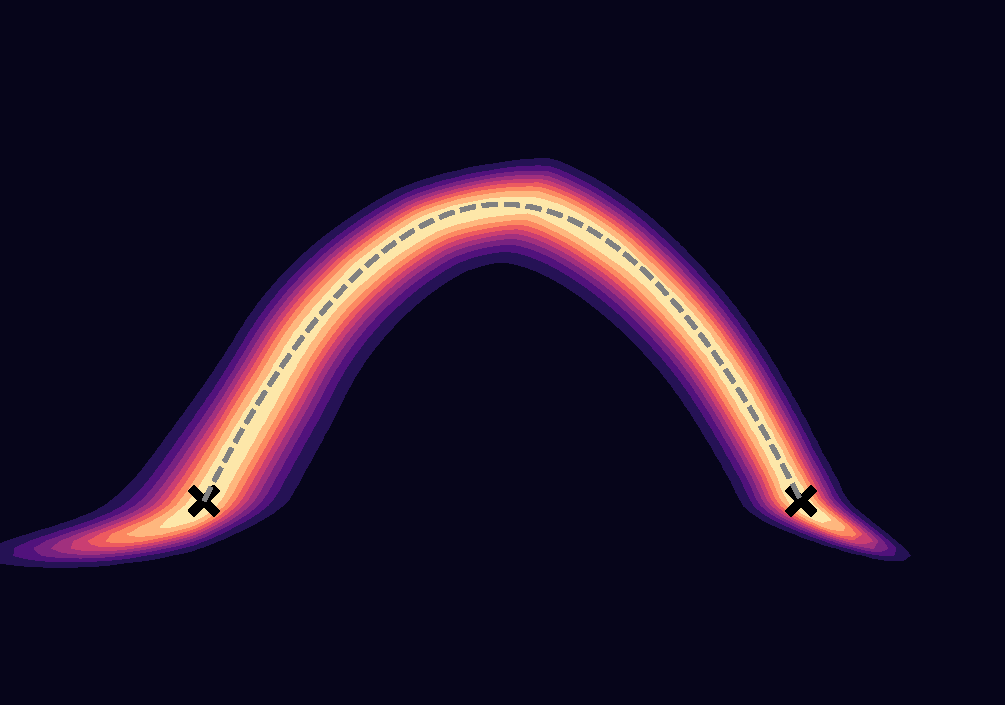
\includegraphics[width=12cm]{plots/mode_connectivity.pdf}
\caption{}
\label{fig_mode_connectivity}
\end{figure}

Even more surprisingly, the loss landscape of deep neural networks contains planes with arbitrary patters, such as images of a bat or a cow. \cite{sightseeing} The complexity of the loss landscape has important consequences for Bayesian neural networks that are discussed in section \ref{sec_results}.

\section{Bayesian neural network}

As described in section \ref{sec_nn_vs_bnn}, a neural network can be used as a likelihood function to represent $p(\tilde{y} | \tilde{x}, \theta)$. In a Bayesian context, we define a prior distribution (belief) over $\theta$ before observing any data, $p(\theta)$, and use this belief together with the likelihood function over a training dataset to obtain a posterior distribution over $\theta$, $p(\theta | x, y)$, as described in Eq. \ref{eq_posterior}. Given this posterior distribution over $\theta$, we can obtain the \textit{posterior predictive distribution} $p(\tilde{y} | \tilde{x}, x, y)$ as described in Eq. \ref{eq_post_pred}. Typically, the posterior predictive distribution is the distribution that we are most interested in. It allows us to perform prediction without conditioning on any particular value of $\theta$.

\subsection{Model uncertainty}

When making a prediction, the total uncertainty in our estimate is a combination of \textit{data uncertainty} and \textit{model uncertainty}. Data uncertainty is the uncertainty over the output variable in any given likelihood function. For example, if we assume that $y \sim N(0, 1)$, the data uncertainty is equal to the variance of the normal distribution. However, in practice, we often don't know what the true distribution generating the data is. For example, it might be $N(0, 1)$, but it could also be $N(0.2, 1.1)$ or $N(0.06, 0.82)$. This is what the term \textit{model uncertainty} refers to. It is the uncertainty in our predictions caused by the fact that we don't know what the true model is.

Let's return to the dataset in Fig. \ref{fig_1d_dataset}. Say we observe the plotted data, $(x, y)$, and we are interested in predicting $\tilde{y}$ given a new observation of $\tilde{x}$ (the accent on $x$ and $y$ is used here to simply distinguish the new observation from the plotted data). We will use an MLP with a single hidden layer of 50 nodes and a $N(0, 0.1^2)$ prior over $\theta$. As before, the network outputs the tuple $(\mu, \sigma^2)$ for each observation and we assume that $y \sim N(y, \sigma^2)$.

The frequentist approach would be to find the MAP solution for $\theta$ and use it to model $p(\tilde{y} | \tilde{x})$. However, there is a crucial problem with this approach. While the obtained model is certainly is going to fit the observed data well, it does not take into consideration the fact that different models might also fit the data similarly well. Hence, it fails to take into consideration any kind of model uncertainty. As a result, its predictions will tend to be \textit{overconfident}, meaning the model will output smaller confidence intervals than it ]ref{should. For example, a $95\%$ confidence interval generated by this model will contain \textit{less} than $95\%$ of the true values, since the interval is too narrow.

The Bayesian approach takes into consideration model uncertainty. When training a BNN, the output is a distribution over $\theta$, rather than just a single value. Hence, the distribution over $\theta$ is a distribution over different models that might describe the data, and the density of the distribution describes our belief about how likely a specific model is.

Fig. \ref{fig_1d_predictions_overlaid} displays the concept of model uncertainty using a standard neural network and a Bayesian neural network. A NN trained using SGD is a single model corresponding to a single value of $\theta$. On the other hand, a BNN comprises a distribution over possible models. The right plot in Fig. \ref{fig_1d_predictions_overlaid} shows the different likelihoods for $y$ obtained by sampling $\theta$ from the posterior. The BNN does what we would intuitively like it to do: it considers that a set of different models might generate the data, and it consider all of them jointly. As we move farther away from observed data along the $x$-axis, the BNN's uncertainty increases, since we are gradually less confident about the behavior of the true model there. Conversely, the NN's confidence \textit{increases} as it moves father away from the observed data, which is undesirable. There is no reason to assume that observation far away from the observed data will continue to follow the same linear trend that it predicts.

\begin{figure}[ht]
\centering
\makebox[\textwidth][c]{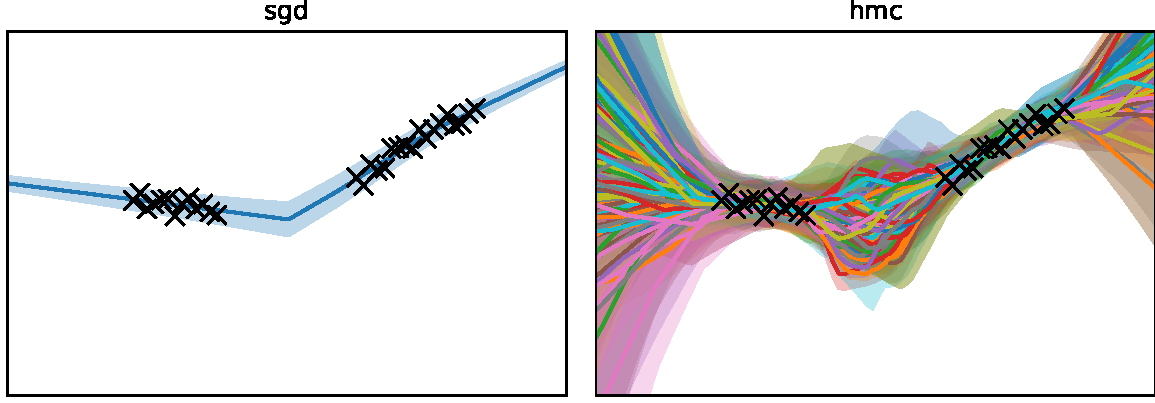
\includegraphics[width=16cm]{plots/1d_predictions_overlaid.pdf}}
\caption{}
\label{fig_1d_predictions_overlaid}
\end{figure}

A more accurate way to visualize the predictions of a BNN is to plots its probability density function (PDF), which requires marginalizing over $\theta$. In general, this cannot be done exactly, but a good approximation is to draw samples from the posterior, $\theta_i$, and average the predictions over these samples. This technique is further described in section \ref{sec_prediction}.

\begin{figure}[ht]
\centering
\makebox[\textwidth][c]{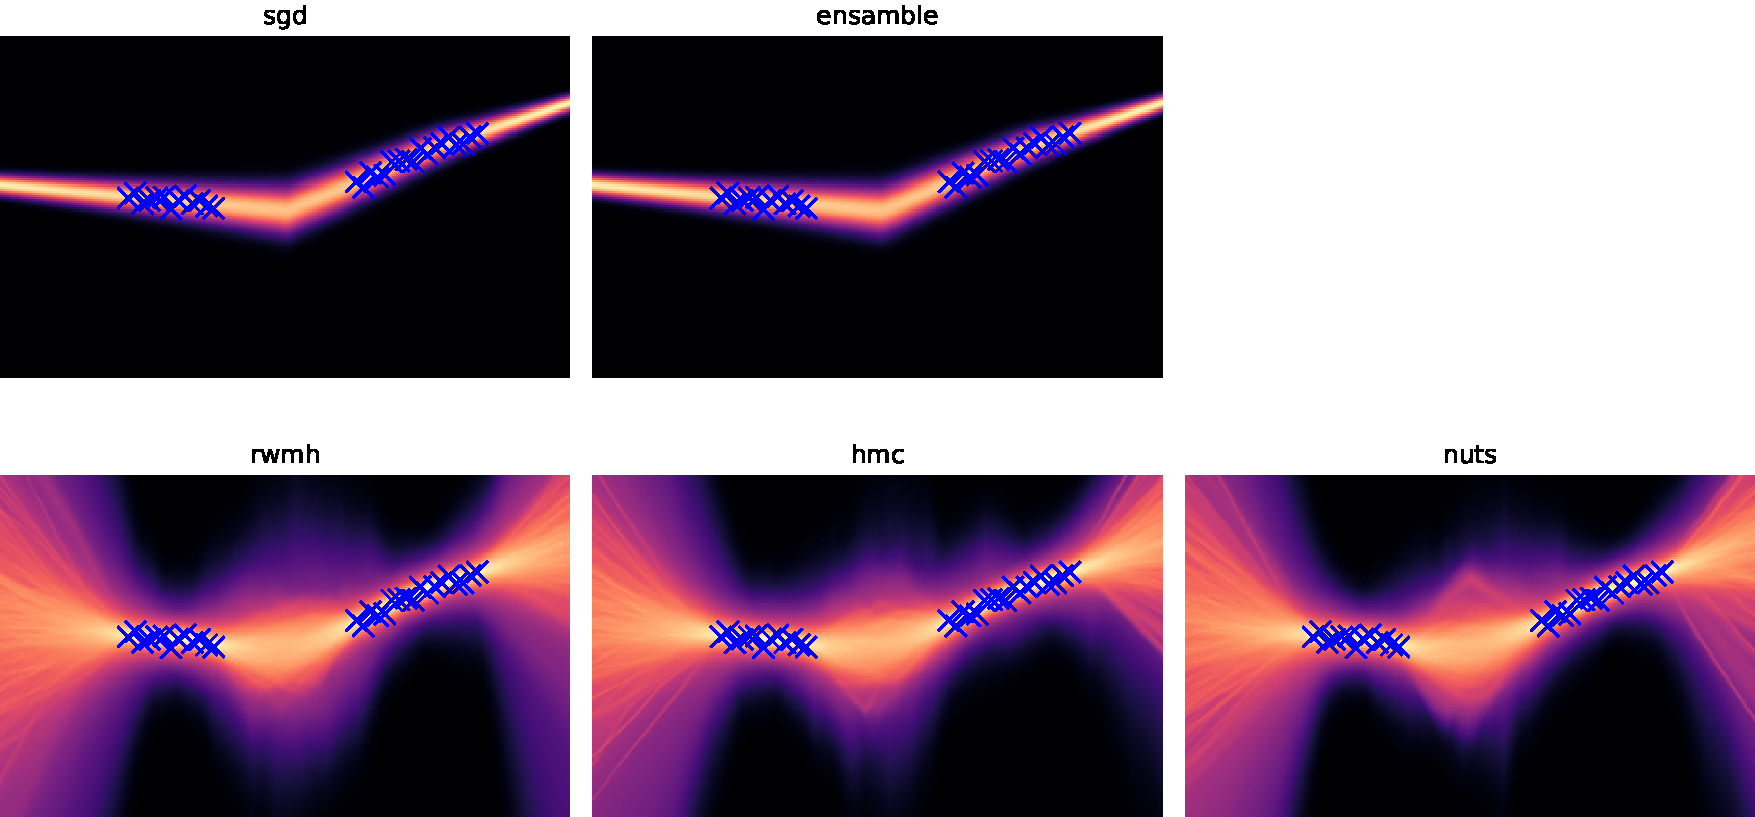
\includegraphics[width=16cm]{plots/1d_predictions_pdf.pdf}}
\caption{}
\label{fig_1d_predictions_pdf}
\end{figure}

A simpler and more common way to visualize the predictions is to plot the confidence interval and mean estimate. One way this can be achieved is to sample $\theta_i$ from the posterior and then sample $y$ from each $\theta_i$. The empirical quantiles of the sampled values of $y$ can then be used to obtain approximate confidence intervals and an approximate mean.

\begin{figure}[ht]
\centering
\makebox[\textwidth][c]{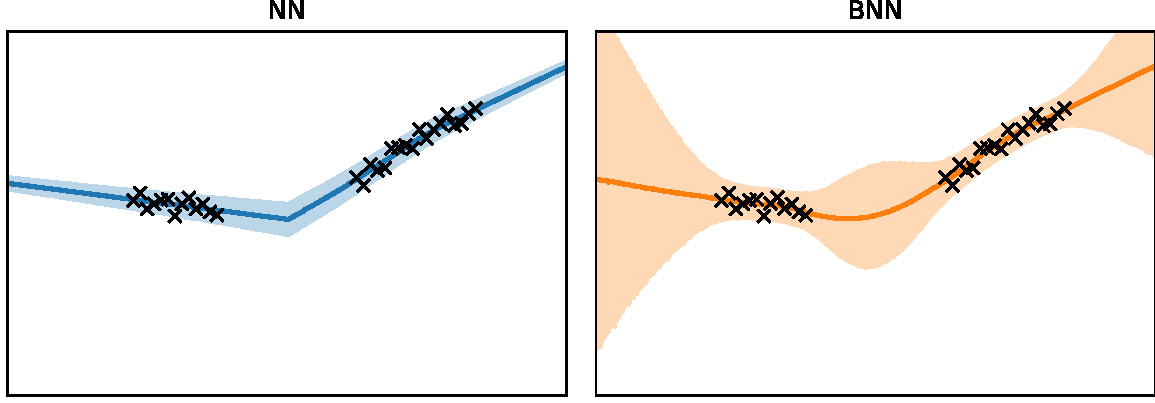
\includegraphics[width=16cm]{plots/1d_predictions_ci.pdf}}
\caption{}
\label{fig_1d_predictions_ci}
\end{figure}

\subsection{Prior selection}

All of the prior examples used the prior distribution $\theta \sim N(0, 0.1^2)$, but this choice is arbitrary. The prior acts as a regularizer, assigning more weight to some models and less weight to others. The goal of a normal prior centered around zero, with a low variance is to favor models with parameters that are small in magnitude. The smaller the magnitude of the weights, the smoother and simpler we expect the likelihood function to be. Conversely, when a neural network has weights that are large in magnitude, it is able to represent functions that are very rough.

Fig. \ref{fig_1d_predictions_by_stdev} shows the posteriors obtained by varying the standard deviation of the prior. We see that a small standard deviation (i.e. an informative prior) acts as a strong regularization. A value of $0.1$ seemingly fails to capture the underlying trend in the observed data, but values $0.2, 0.5, 1, 3$ all seem reasonable. We might favor values $0.2$ and $0.5$ when we expect the underlying data generating process to be simple -- we expect that any observed trend in the data would continue to hold even for unobserved values of $x$. Values $1$ and $3$, on the other hand, represent an increased model uncertainty -- even though the observed values of $x$ have a certain trend, there might be a different trend for unobserved values of $x$. A standard deviation of $10$ takes this to the extreme, representing the belief that we cannot say almost anything at all about the trend for unobserved values of $x$. This behavior of the posterior predictive distribution in a BNN is analogous to Gaussian processes. In fact, in the infinite-width limit, some BNNs become a Gaussian process. \cite{neural_tangents}

\begin{figure}[ht]
\centering
\makebox[\textwidth][c]{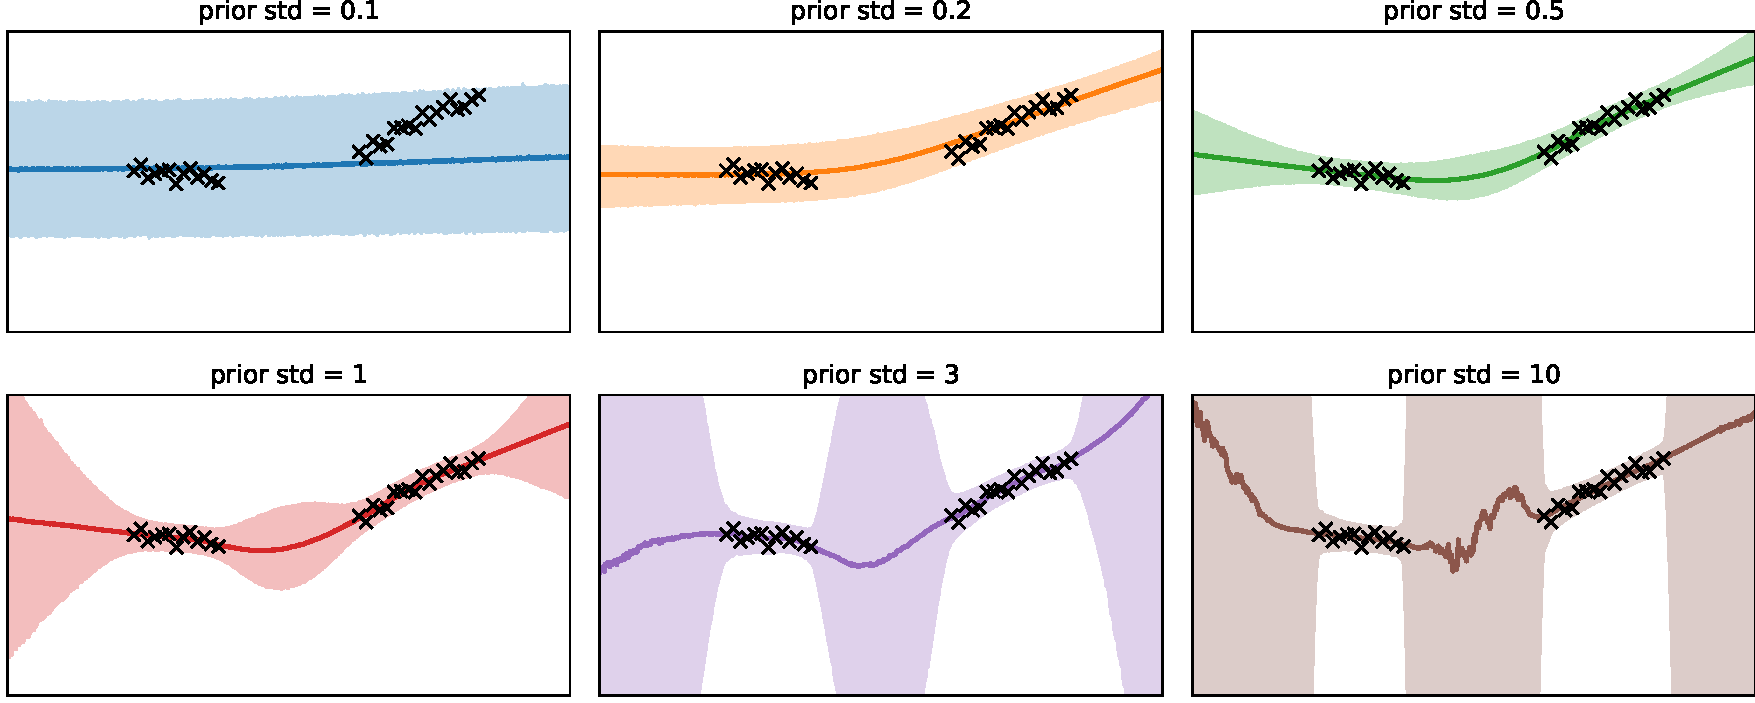
\includegraphics[width=18cm]{plots/1d_predictions_by_stdev.pdf}}
\caption{}
\label{fig_1d_predictions_by_stdev}
\end{figure}

\subsection{Prediction}
\label{sec_prediction}

The distribution over the response variable $\tilde{y}$, given a new observation $\tilde{x}$ and training data $(x, y)$ is given by the \textit{posterior predictive distribution} $p(\tilde{y} | \tilde{x}, x, y)$, derived in Eq. \ref{eq_post_pred}. This equation involves integrating over $\theta$, which has the same number of dimensions as the number of parameters of the neural network, meaning possibly millions or billions. In general, the integral doesn't have a closed-form solution and numerical methods must be used to approximate it.

In low dimensions, the \textit{trapezoidal rule} is an intuitive method to numerically compute an integral:

\begin{equation}
\int_{a}^{b} f(x) d x \approx \frac{1}{2}(b-a)(f(a)+f(b))
\end{equation}

However, let's say that we need to use $n$ trapezoids to approximate a $1D$-integral. Then, as the number of dimensions $d$ grows, the number of trapezoids required grows like $n^d$, i.e. exponentially. With anything but a tiny neural network, this method is infeasible.

\textit{Monte Carlo simulation} is a better approach. We express the integral as an expectation over some probability distribution $p(x)$, draw samples from $p(x)$, and compute the empirical mean of $f(x)$ over the samples:

1. sample $x_i \sim p(x)\\$
2. $\int f(x)p(x) dx = E_x[f(x)] \approx \hat{f}_n = \frac{1}{n} \sum_{i=1}^n f(x_i)$

Using the strong law of large numbers and assuming $x_i$ are i.i.d.:

\begin{equation}
\mathbb{P}\left(\lim_{n \rightarrow \infty} \hat{f}_n=\mathbb{E}_{\pi}[f]\right)=1
\end{equation}

In other words, we can use $n$ i.i.d. samples from $p(x)$ to approximate $\int f(x)p(x) dx$. As $n \rightarrow \infty$, this approximation will converge almost surely to the true value of the integral. Even better, by using the central limit theorem, we get that the approximation converges as $1/\sqrt n$, i.e., its convergence rate does not depend on the number of dimensions. This is a crucial property to work in high dimensions.

% TODO: correlation ⇒ worse MC estimate

We can apply this technique to the posterior predictive distribution of a BNN by taking the expectation of the likelihood $p(\tilde{y}|\tilde{x},\theta)$ over the posterior $p(\theta|x,y)$. However, we must be careful about how this simulation is implemented. As described in section \ref{sec_loss_fn}, computers struggle to work with small numbers, which is why working with the logarithms of probabilities is more accurate. Unfortunately, we cannot average over $\log p(\tilde{y})$ directly, rather we must average over $p(\tilde{y})$. The naive solution would be to simply exponentiate $\log p(\tilde{y})$, but since $p(\tilde{y})$ may be close to zero, this would result in underflow. A better solution is to use the $\textrm{LogSumExp}$ function, which is a stable way to compute the logarithm of a sum of exponents. The resulting expression is derived below:

\begin{align}
\begin{split}
p(\tilde{y}) &= E_\theta [p(\tilde{y}, \theta)] \\
p(\tilde{y}) &\approx \sum p(\tilde{y}|\theta_i) p(\theta_i) \\
p(\tilde{y}) &\approx \sum p(\tilde{y}|\theta_i) \frac{1}{n} \\
p(\tilde{y}) &\approx \sum \exp \log p(\tilde{y}|\theta_i)) \frac{1}{n} \\
\log p(\tilde{y}) &\approx \log(\sum \exp \log p(\tilde{y}|\theta_i) \frac{1}{n}) \\
\log p(\tilde{y}) &\approx \textrm{LogSumExp} (\log p(\tilde{y}|\theta_i)) - \log(n)
\end{split}
\end{align}

Hence, all we need is to find an efficient method to sample the posterior. When the likelihood function has a simple form, and with a bit of luck, there may exist a \textit{conjugate prior} distribution such that the posterior distribution belongs to the same family of distributions as the prior. This is useful trick because it allows us to obtain the exact posterior distribution with negligible computational expense. However, neural networks are so complex that they do not have any known useful conjugate priors. Instead, to obtain the posterior, we must choose one of two approaches: \textit{variational inference} or \textit{MCMC-based sampling}. Both of these methods only provide approximations to the posterior distribution and come with their own unique tradeoffs. These are discussed below in sections \ref{sec_vi} and \ref{sec_mcmc}.

\subsection{Variational inference}
\label{sec_vi}

First, we could approximate the true posterior distribution using a simpler distribution from which we can easily draw samples. While the approximation may be inaccurate, we can often fit the simpler distribution with little computational expense. Hence, this is good approach if we are willing to trade off accuracy for compute. It is called \textit{variational inference}.

\subsubsection{SWAG}
% TODO: write about MFVI instead

Stochastic Weight Averaging Gaussian (SWAG) is an efficient way to compute a Gaussian approximation around the maximum a posteriori (MAP) estimate. \cite{swag} It introduces little computational overhead over conventional SGD training and improves both accuracy and calibration. \cite{swag}

If we consider the geometry of the loss function around the MAP solution to be approximately Gaussian, we can exploit the SGD trajectory to fit this Gaussian approximation. The idea is that as SGD converges to the MAP solution, it will bounce around the minimum. We can take the sample of parameters after each SGD training epoch to fit a Gaussian approximation of the loss function. Since the loss function is proportional to the log-posterior distribution, the fitted Gaussian distribution is a local Gaussian approximation of the posterior around the MAP solution.

The main limitation of SWAG is that it only describes a single mode of log-posterior distribution. As shown in section \ref{sec_loss_landscape}, the posterior distribution of neural networks is multi-modal. In deep neural networks, the the distributions described by each mode tend to differ in function space, so a local approximation around a single mode fails to capture the functional diversity of the posterior. \cite{deep_ens}

\subsubsection{Deep ensembles}

One model that takes into account the multi-modality of the posterior is a \textit{deep ensemble}. It consists of training a set of independent neural networks using SGD, where each network is initialized with different parameters and hence converges to a different mode of the posterior, and then averaging their predictions. Another way of describing this model is that the posterior over $\theta$ is a uniform categorical distribution over the independent SGD solutions.

In section \ref{sec_loss_landscape}, Fig. \ref{fig_1d_ens_predictions} shows the predictions of each network in a six-network ensemble trained on a tiny regression dataset. In the figure, each network appears identical in function space, even though the parameters of each network are different. However, deeper neural networks have different behavior. In deep NNs, each mode of the posterior tends to differ from the other modes in function space. \cite{deep_ens}

Empirically, a deep ensemble is more faithful approximation to the true posterior of a BNN than SWAG. \cite{bnn_posterior} Point estimates of multiple modes capture more of the functional diversity of the posterior than a local approximation around a single mode. Deep ensembles are very popular in practice, as they are simple and provide a significant increase in accuracy compared to SGD or SWAG. \cite{multiswag}

\subsection{Markov chain Monte Carlo}
\label{sec_mcmc}

In variational inference, we work with the posterior distribution by approximating it using a simpler distribution. In order to avoid the approximation, we must directly draw samples from the true posterior distribution, as described in Eq. \ref{eq_posterior}.

\textit{Markov chain Monte Carlo} (MCMC) is a family of universal methods for drawing samples from a probability distribution. When applied to the posterior of a BNN, they allow us to draw (correlated) samples from the true posterior distribution, without having to approximate it using a simpler distribution.

The idea behind MCMC is to create a \textit{Markov chain} that has an equilibrium distribution equal to the posterior distribution that we want to draw samples from -- we will call this distribution the \textit{target distribution}.

A Markov chain is any sequence of random variables $\theta_i$ that satisfies the Markov property: the probability of moving to the next state ($t+1$) depends only on the current state ($t$) and not on the previous states ($1 \ldots t$). Eq. \ref{eq_markov_propery} defines this property formally.

\begin{equation}
p(\theta_{t+1}|\theta_1,\ldots \theta_t)=p(\theta_{t+1}|\theta_t)
\label{eq_markov_propery}
\end{equation}

In MCMC, we define a process which satisfies the markov property and thus when we draw samples from it, we get a Markov chain. We define the process by its \textit{transition kernel}, which is the probability distribution over the next state given the current state, $p(\theta_{t+1}|\theta_t)$. We will only focus on time-homogeneous chains, where the transition kernel doesn't change over time.

In order to draw samples $\theta_0 \ldots \theta_{n-1}$ from a Markov chain defined by the transition kernel $p(\theta_{t+1}|\theta_t)$, we use the following algorithm:

\begin{algorithm}
\caption{Metropolis-Hastings}
\label{alg_mh}
\begin{algorithmic}
\State $\theta_0 \gets \theta_{\textrm{init}}$
\For{$i \gets 1 \ldots n_\textrm{samples}$} 
	\State resample $\theta_i \sim p(\theta_i|\theta_{i-1})$
\EndFor
\end{algorithmic}
\end{algorithm}

The goal is to define a process whose unique \textit{equilibrium distribution} is equal to the target distribution $\pi(\theta)$ that we want to draw samples from. This means that for any $\theta_0$, as $n \rightarrow \infty$, $p(\theta_n|\theta_0) \xrightarrow{d} \pi(\theta)$. This property will be met iff the chain is \textit{$\pi$-irreducible}, \textit{aperiodic}, and \textit{$\pi$-invariant}.

A chain is $\pi$-irreducible iff any state $x$ that has a non-zero probability in the target distribution $\pi(\theta) > 0$ can be reached from any other state of the chain $\theta_0$ in a finite number of steps $n$:

\begin{equation}
\pi(\theta) > 0 \Rightarrow \exists \ n, \ p(\theta_n = \theta|\theta_0) > 0
\end{equation}

A chain is periodic if it has a state $\theta$ s.t. the return to this state can only happen in a multiple of $k$ steps, where $k > 1$. In all of the Markov chains that we consider, it is possible to transition from any state to any other state in a single step. This implies that the chains are \textit{both} $\pi$-irreducible \textit{and} aperiodic.

The last property that the Markov chain needs to meet is $\pi$-invariance. It means that once we reach the equilibrium state of the chain, the chain will remain in the equilibrium:

\begin{equation}
\theta_t \sim \pi(\theta) \Rightarrow \theta_{t+1} \sim \pi(\theta)
\end{equation}

Let's denote our target posterior distribution as $\pi(\theta)$. Then, once we define a $\pi$-irreducible, aperiodic, and $\pi$-invariant chain, running algorithm \ref{alg_mh} will yield samples that are asymptotically distributed as the posterior.

\subsubsection{Metropolis-Hastings}

The simplest and most common MCMC algorithm is \textit{Metropolis-Hastings}. It is a general family of algorithms that ensure $\pi$-invariance. Two out of the three MCMC algorithms discussed in this essay belong to this family.

First, let's denote two arbitrary states in $\pi(\theta)$ as $\theta$ and $\theta'$. Next, let's define a \textit{proposal distribution} $Q(\theta'|\theta)$ and \textit{acceptance probability} $A(\theta'|\theta)$. When $\theta' \ne \theta$, the transition \textit{density} is equal to the product of the proposal density and the acceptance probability, as described in Eq. \ref{eq_transition_prob}. The event $\theta' = \theta$ happens with \textit{probability mass} $1-\int_{-\infty}^{\infty} Q(\theta'|\theta)A(\theta'|\theta) d\theta'$ .

\begin{equation}
p(\theta'|\theta) = Q(\theta'|\theta)A(\theta'|\theta)
\label{eq_transition_prob}
\end{equation}

One way to satisfy $\pi$-invariance is to make the probability of observing state $\theta$ followed by state $\theta'$ is the same as $\theta'$ followed by $\theta$. This condition is called \textit{detailed balance} / \textit{reversibility} and is defined in Eq. \ref{eq_detailed_balance}.

\begin{align}
\begin{split}
p(\theta'|\theta)\pi(\theta) &= p(\theta|\theta')\pi(\theta') \\
\frac{p(\theta'|\theta)}{p(\theta|\theta')} &= \frac{\pi(\theta')}{\pi(\theta)} \\
\frac{Q(\theta'|\theta)A(\theta'|\theta)}{Q(\theta|\theta')A(\theta|\theta')} &= \frac{\pi(\theta')}{\pi(\theta)} \\
\frac{A(\theta'|\theta)}{A(\theta|\theta')} &= \frac{Q(\theta|\theta')\pi(\theta')}{Q(\theta'|\theta)\pi(\theta)}
\label{eq_detailed_balance}
\end{split}
\end{align}

By setting $A(\theta'|\theta)$ to the value defined in Eq. \ref{eq_accept_prob}, we ensure that detailed balance (Eq. \ref{eq_detailed_balance}) always holds, hence our chain is $\pi$-invariant. 

\begin{equation}
A(\theta'|\theta) := \min \left(1, \frac{Q(\theta|\theta')\pi(\theta')}{Q(\theta'|\theta)\pi(\theta)} \right)
\label{eq_accept_prob}
\end{equation}

The different flavor of Metropolis-Hastings differ only in their proposal distribution $Q(\theta'|\theta)$. The acceptance probability is always the one defined in Eq. \ref{eq_accept_prob}. A very useful property of this acceptance probability is that $\pi(\theta)$ needs to be known only up to a multiplicative constant. The posterior, as defined in Eq. \ref{eq_posterior} involves an intractable integral over $\theta$, which has potentially millions of dimensions. Fortunately, the value of this integral is constant w.r.t. $\theta$, so it cancels out in Eq. \ref{eq_accept_prob}. Hence, when working with $\pi(\theta)$, we can evaluate it as a product of the likelihood multiplied by the prior, without having to compute the evidence.

The samples drawn by MCMC are dependent, by the nature of a Markov chain. However, in order to get a good approximation of the posterior predictive distribution, as described in section \ref{sec_prediction}, we would ideally like the samples to be uncorrelated. The reason behind this is that a high autocorrelation of samples implies that the chain explores the posterior slowly. If the chain is currently in $\theta$, subsequent samples from the chain will still be close to $\theta$, rather than exploring the full distribution. A different view on this is that we would prefer the chain to have a large average step size between each of its samples. In order to achieve this, we must design a proposal distribution that proposes large steps that have a high acceptance probability.

\subsubsection{Random-walk Metropolis-Hastings}

The simplest Metropolis-Hastings algorithm is the \textit{Random-walk Metropolis-Hastings} (RWMH). In RWMH, the proposal distribution over $\theta'$ is a normal distribution centered around $x$: $Q(\theta'|\theta) \sim N(\theta, \sigma^2)$. A useful property of the normal distribution is that its density at $\theta$ only depends on the distance of $\theta$ from the mean of the distribution. As a result, $Q(\theta'|\theta) = q(\theta|\theta')$, so Eq. \ref{eq_accept_prob} simplifies to Eq. \ref{eq_rwmh_accept_prob}. The left side of Fig. \ref{fig_rwmh_vs_hmc} illustrates the RWMH algorithm.

\begin{equation}
A(\theta'|\theta) = \min \left(1, \frac{\pi(\theta')}{\pi(\theta)} \right)
\label{eq_rwmh_accept_prob}
\end{equation}

\begin{figure}[ht]
\centering
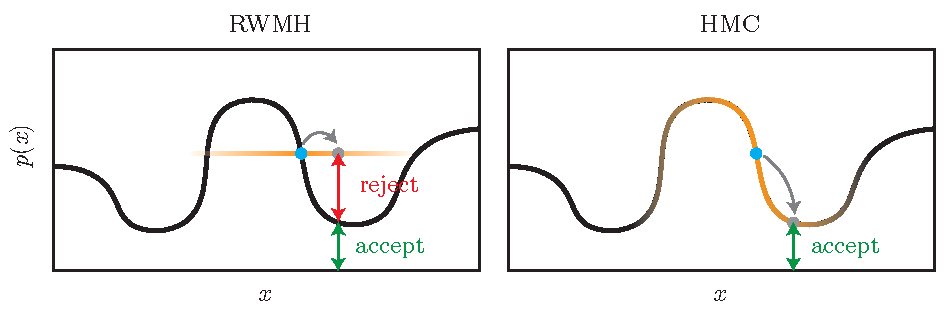
\includegraphics[width=14cm]{illustrations/rwmh_vs_hmc.pdf}
\caption{An illustration of Random-walk Metropolis-Hastings (RWMH) on the left and Hamiltonian Monte Carlo (HMC) on the right. The current state is represented by the blue point and the proposal distribution is illustrated by the yellow line. In RWMH, the proposal's acceptance probability depends on the height difference between the proposal and the target distribution. If the proposal is significantly higher than the target distribution, it will likely get rejected. If it is lower, it will always get accepted. Meanwhile, HMC proposes samples that lie exactly on the target distribution, so they always get accepted.}
\label{fig_rwmh_vs_hmc}
\end{figure}

The only hyperparameter of the RWMH algorithm is the covariance matrix of the proposal distribution, $\sigma^2$. The simplest choice for the covariance matrix is a constant multiplied by the identity matrix, meaning the proposals for each component are independent and have the same variance. While under some conditions, there might exist better choices of $\sigma^2$, in different conditions, these might be inferior to the simple independent proposals with constant variance. Hence, for simplicity, we will only focus on independent proposals with constant variance. Hence, the only hyperparameter that remains is a single number that represents the standard deviation of each dimension of the proposal distribution -- this is called the \textit{step size}.

Setting the step size too low will result in tiny steps that always get accepted. Setting it too high will result in large steps that always get rejected. So there always exists an optimum step size which offers the best tradeoff between these qualities. In high dimensions, the optimum step size is the one that results in roughly ==TODO== acceptance probability. ==TODO: CITATION==. Proving this result is beyond the scope of this essay.

The complete RWMH algorithm is described below:
\begin{algorithm}
\caption{RWMH}
\label{alg_rwmh}
\begin{algorithmic}
\For{$\textrm{step} \gets 1 \ldots n_\textrm{samples}$} \Comment{generate $n_\textrm{samples}$ from target distribution}
	\State resample $\theta' \sim N(\theta, \sigma^2)$ \Comment{propose new parameters}
	\State with prob. $\min{(1, \frac{\pi(\theta')}{\pi(\theta)})}$, set $\theta \gets \theta'$ \Comment{accept / reject the proposal}
\EndFor
\end{algorithmic}
\end{algorithm}

\subsubsection{Hamiltonian Monte Carlo}

Hamiltonian Monte Carlo (HMC) exploits the geometry of the target distribution to propose arbitrarily large steps with acceptance probability exactly equal to one. \cite{hmc} This is illustrated on the right side of Fig. \ref{fig_rwmh_vs_hmc}.

The idea is that instead of drawing samples directly from our target distribution $\pi(\theta)$, we define a new variable $v$, called the \textit{momentum}, and we draw samples from the joint distribution $\pi(\theta, v) := \pi(\theta)\pi(v)$. Once we have the joint samples $(\theta, v)$, we can discard the momentum $v$ and we are left with samples from our target distribution $\theta$.

HMC alternates between updating the momentum $v$ on its own and jointly updating the position together with the momentum $(\theta, v)$. Both of these updates are performed in a Metropolis-Hastings fashion. We will denote the current values as $\theta, v$ and the proposed values as $\theta', v'$.

When the momentum is updated on its own, it is simply drawn from a normal distribution centered around zero, $v' \sim N(0, \sigma^2)$. Also, by design, the proposal distribution of $v$ is equal to the target distribution of $v$: $Q(v) \overset{d}{=} \pi(v)$. Using the formula for acceptance probability from Eq. \ref{eq_accept_prob}, we see that the proposal always gets accepted:

\begin{align}
\begin{split}
A(\theta,v'|\theta,v) &= \min \left(1, \frac{Q(\theta,v|\theta,v')\pi(\theta,v')}{Q(\theta,v'|\theta,v)\pi(\theta,v)} \right) \\
&= \min \left(1, \frac{Q(v)\pi(\theta)\pi(v')}{Q(v')\pi(\theta)\pi(v)} \right) \\
&= \min \left(1, \frac{Q(v)\pi(v')}{Q(v')\pi(v')} \right) \\
&= 1
\end{split}
\end{align}

The joint proposal for $(\theta, v)$ is more complicated. In order to understand it, it helps to think of $(\theta, v)$ as the state of a physical particle rolling along a hill. $\theta$ is the particle's position, $v$ is its momentum, and the shape of the hills is described by the target distribution. When we updated the particle's momentum, it was like flicking it in a random direction. In order to update its position and momentum together, we will simply let the particle roll for a while and then we will record its new position and momentum. The whole system is designed in such a way that no matter where the particle ends up, its new position and momentum will get accepted will probability one.

First, we need to define some quantities: $U(\theta)$ -- the \textit{potential energy} of the particle, $K(v)$ -- the \textit{kinetic energy} of the particle, and $H(\theta, v)$ -- the \textit{Hamiltonian} of the particle:

\begin{align}
\begin{split}
U(\theta) &= -\log \pi(\theta) \\
K(v) &= \frac{1}{2} ||v||^2 \\
H(\theta, v) &= U(\theta) + K(v)
\end{split}
\label{eq_hamiltonian}
\end{align}

Following the above equations, we can derive the relationship between the Hamiltonian and the target distribution:

\begin{align}
\begin{split}
H(\theta, v) &= -\log \pi(\theta) + \frac{1}{2}||v||^2 \\
\pi(\theta, v) &= \exp {-H(\theta, v)} \\
&= \exp \left(\log \pi(\theta) - \frac{1}{2}||v||^2 \right) \\
&= \pi(\theta) \frac{1}{2}||v||^2 \\
&\propto \pi(\theta) \pi(v)
\end{split}
\end{align}

When particle's state evolves through \textit{Hamiltonian dynamics}, the particle's Hamiltonian is conserved, meaning that the density of the target distribution is conserved. Hamiltonian dynamics are defined by the following equations:

\begin{align}
\begin{split}
\frac{d\theta}{dt} &= \frac{\partial H}{\partial v} \\
\frac{dv}{dt} &= -\frac{\partial H}{\partial \theta}
\end{split}
\label{eq_ham_dynamics}
\end{align}

Additionally, Hamiltonian dynamics are time-reversible, so $Q(\theta',v'|\theta,v) = Q(\theta,v|\theta',v')$ and they preserve volume, so the ratio of probabilities before and after the transformation is the same as the ratio of probability densities . These properties, combined with the fact that the Hamiltonian is conserved, implies that the acceptance rate of the new state $(\theta', v')$ is exactly one:

\begin{align}
\begin{split}
A(\theta',v'|\theta,v) &= \min \left(1, \frac{Q(\theta,v|\theta',v')\pi(\theta',v')}{Q(\theta',v'|\theta,v)\pi(\theta,v)} \right) \\
&= 1
\end{split}
\end{align}

Unfortunately, Eq. \ref{eq_ham_dynamics} are differential equations that cannot be computed exactly -- they must be numerically approximated. As a result, the Hamiltonian is not perfectly conserved, hence the true acceptance probability is close to one, but not exactly one:

\begin{align}
\begin{split}
A(\theta',v'|\theta,v) &= \min \left(1, \frac{Q(\theta,v|\theta',v')\pi(\theta',v')}{Q(\theta',v'|\theta,v)\pi(\theta,v)} \right) \\
&= \min \left(1, \frac{\pi(\theta',v')}{\pi(\theta,v)} \right) \\
&= \min \left(1, \frac{\exp -H(\theta',v')}{\exp -H(\theta,v)} \right) \\
&= \min \left(1, \exp \left(-H(\theta', v') + H(\theta, v) \right) \right) \\
&= \min \left(1, \exp \left(\log \pi(\theta') - \frac{1}{2}||v'||^2 -\log \pi(\theta) + \frac{1}{2}||v||^2 \right) \right) \\
&= \min \left(1, \frac{\pi(\theta')}{\pi(\theta)} \exp \left( \frac{1}{2}||v||^2 - ||v'||^2 \right) \right)
\end{split}
\label{eq_hmc_accept_prob}
\end{align}

In order to get the acceptance probability as close to one as possible, we must use an efficient way to simulate Hamiltonian dynamics, as described in Eq. \ref{eq_ham_dynamics}. A standard way to simulate differential equations is Euler’s method:

\begin{align}
\begin{split}
v_t &\leftarrow v_t + \varepsilon \frac{dv_t}{dt}(t) = v_t - \varepsilon \frac{\partial U}{\partial \theta}(\theta_t) \\
\theta_t &\leftarrow \theta_t + \varepsilon \frac{d\theta_t}{dt}(t) = \theta_t - \varepsilon v_t
\end{split}
\end{align}

However, there exists a significantly more accurate method to simulate Hamiltonian dynamics: the leapfrog algorithm. \cite{hmc} First, we do a half-step update of the momentum, then a full update of the position (using the new momentum value), and finally another half-step update of the momentum (using the new position).

\begin{align}
\begin{split}
v_{t+\varepsilon/2} &\leftarrow v_t - \frac{\varepsilon}{2} \frac{\partial U}{\partial \theta}(\theta_t) \\
\theta_{t+\varepsilon} &\leftarrow \theta_t + v_{t+\varepsilon/2} \\
v_t &\leftarrow v_{t+\varepsilon/2} - \frac{\varepsilon}{2} \frac{\partial U}{\partial \theta}(\theta_{t+\varepsilon})
\end{split}
\label{eq_leapfrog}
\end{align}

Conveniently, each transformation in Eq. \ref{eq_leapfrog} is a shear transformation, so the leapfrog algorithm preserves volume exactly. Also, the algorithm is time-reversible by negating $v$, running it for the same number of steps, and negating $v$ again. Both of these properties are required for Eq. \ref{eq_hmc_accept_prob} to hold. \cite{hmc}

In general, HMC has three hyperparameters: step size $\sigma$, number of leapfrog steps $n$, and \textit{mass matrix} $m$. For simplicity, we only consider the use of a unit mass matrix, meaning we don't have to include it in any equations. Under some conditions, using a non-unit mass matrix might be beneficial, as it means that the momentum is updated at different rates for each parameter. However, there is no universally optimum value of the mass matrix.

The product of step size with the number of steps is called the \textit{trajectory length}. It dictates the average arc length that the particle travels during Hamiltonian dynamics. If the trajectory length is too small, the particle will make tiny steps, resulting in highly correlated samples of $\theta$. On the other hand, if the trajectory length is too large, the particle might repeatedly oscillate around its origin, as if it were rolling around the trough of a deep valley. This idea is further discussed in section \ref{sec_nuts}. In practice, we might set the trajectory length roughly similar to what we would expect the standard deviation of the posterior to be. \cite{bnn_posterior} This is simple to estimate when the prior dominates the likelihood, but harder when the likelihood dominates the prior.

The computational complexity of HMC scales linearly with the number of steps. Hence, given a fixed trajectory length, we would prefer the step size to be as large as possible. However, as the step size increases, the leapfrog approximation error increases, which reduces the acceptance rate. The solution is to use a step size as large as possible while maintaining a good acceptance rate -- e.g. $80\%$. \cite{bnn_posterior}

The complete HMC algorithm is described below:
\begin{algorithm}
\caption{Leapfrog}
\label{alg_leapfrog}
\begin{algorithmic}
\For{$i \gets 1 \ldots n_\mathrm{steps}$} \Comment{do $n_\mathrm{steps}$ steps}
\State $v \gets v - \frac{\varepsilon}{2} \frac{\partial U}{\partial \theta}$ \Comment{do a half-step update of momentum}
\State $\theta \gets \theta + v$ \Comment{do a full-step update of parameters}
\State $v \gets v - \frac{\varepsilon}{2} \frac{\partial U}{\partial \theta}$ \Comment{do a half-step update of momentum}
\EndFor
\end{algorithmic}
\end{algorithm}

\begin{algorithm}
\caption{HMC}
\label{alg_hmc}
\begin{algorithmic}
\For{$\textrm{step} \gets 1 \ldots n_\textrm{samples}$} \Comment{generate $n_\textrm{samples}$ from target distribution}
	\State resample $v \sim N(0, \sigma^2)$ \Comment{resample momentum}
	\State $\theta', v' \gets \textrm{Leapfrog}(\theta, v)$ \Comment{propose new parameters}
	\State with prob. $\min{\left(1, \frac{\pi(\theta')}{\pi(\theta)} \exp \left( \frac{1}{2}||v||^2 - ||v'||^2 \right) \right)}$, set $\theta \gets \theta'$ \Comment{accept / reject the proposal}
\EndFor
\end{algorithmic}
\end{algorithm}

\subsubsection{No-U-Turn Sampler}
\label{sec_nuts}

The \textit{No-U-Turn Sampler} (NUTS) is a modification of HMC that adapts the trajectory length (by adapting the number of steps) depending on the local geometry of the target distribution. \cite{nuts} The idea is to always run Hamiltonian dynamics \textit{just long enough} -- until the point when running the simulation for any longer would result in the particle moving \textit{closer} to its origin, rather than away from it. Let $(\theta, v)$ denote the state of the particle at the start of Hamiltonian dynamics and $(\theta', v')$ denote the current state of the particle under Hamiltonian dynamics.

We can measure the distance of $\theta'$ to $\theta$ as $||\theta'-\theta||^2$, so the stopping condition is $\frac{d}{dt} ||\theta'-\theta||^2 < 0$. When the stopping condition is reached, we say that the particle makes a \textit{U-turn}. The stopping condition can be expressed in terms of $\theta', \theta, v'$ as derived below:

\begin{align}
\begin{split}
\frac{d}{dt} ||\theta'-\theta||^2 &< 0 \\
\frac{d}{dt} \left((\theta'-\theta) \cdot (\theta'-\theta) \right) &< 0 \\
2(\theta'-\theta) \cdot \frac{d}{dt}(\theta'-\theta) &< 0 \\
(\theta'-\theta) \cdot v' &< 0
\end{split}
\label{eq_uturn}
\end{align}

It would be convenient to simply leapfrog until the particle makes a U-turn and then use the last leapfrog step as the proposal for ($\theta, v$). However, this could create a scenario where a particle traveling forwards in time stops at a different location that a particle traveling backwards in time, thus breaking detailed balance. Fig. \ref{fig_nuts_uturn_detailed_balance} illustrates one such scenario. In order to satisfy detailed balance, we must make sure that the probability of proposing $(\theta, v) \rightarrow (\theta', v')$ is the same as $(\theta', v') \rightarrow (\theta, v)$. In HMC, this was satisfied by running the (time-reversible) leapfrog algorithm for a fixed number of steps. In order for NUTS to stop when it detects a U-turn \textit{and} preserve detailed balance, it needs to operate in a more complicated fashion.

\begin{figure}[ht]
\centering
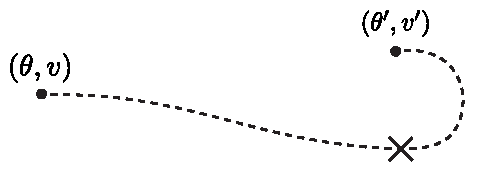
\includegraphics[width=8cm]{illustrations/nuts_uturn_detailed_balance.pdf}
\caption{If a particle travels from $(\theta, v)$ along the dashed leapfrog trajectory, it will make a U-turn at the point $(\theta', v')$. However, if the particle started at $(\theta', v')$ and went backwards in time, it would make a U-turn at the point denoted by a large cross, not at the original starting point $(\theta, v)$.}
\label{fig_nuts_uturn_detailed_balance}
\end{figure}

NUTS works by recursively growing a balanced binary tree. First, we start with the initial position, pick a random direction (forwards or backwards) and leapfrog 1 step. Then, we again choose a random direction (forwards or backwards) and leapfrog 2 steps. Then, we choose a random direction and leapfrog 4 steps... in general, at iteration $i$, we chose a random direction and leapfrog $2^i$ steps. This process continues until we reach a U-turn.

This process implicitly grows a binary tree, where each leaf represents a single state of the particle ($\theta', v'$). At each iteration of NUTS, the size of the tree is doubled: it either grows forwards or backwards by $2^i$ leafs. When the tree is grown forwards, we leapfrog forwards in time starting from the rightmost state $(\theta_\text{right}, v_\text{right})$ and append the new states to the right side of the tree. When the tree is grown backwards, we leapfrog backwards in time, starting from the leftmost state $(\theta_\text{left}, v_\text{left})$ and sequentially append the new states to the left side of the tree. The leafs of the binary tree are always indexed as $0 \ldots (n-1)$, from left to right, where $n$ is the number of leafs in the tree. This means that the index of a given leaf can change as the tree grows, since the leaf's distance from the leftmost leaf can change. Even though we alternate between growing the binary tree forwards and backwards, the resulting tree will be a consistent leapfrog path, i.e. running the leapfrog algorithm from $(\theta_\text{left}, v_\text{left})$ will always reach $(\theta_\text{right}, v_\text{right})$. Fig. \ref{fig_nuts_tree} illustrates the binary tree created after the fifth iteration of NUTS.

\begin{figure}[ht]
\centering
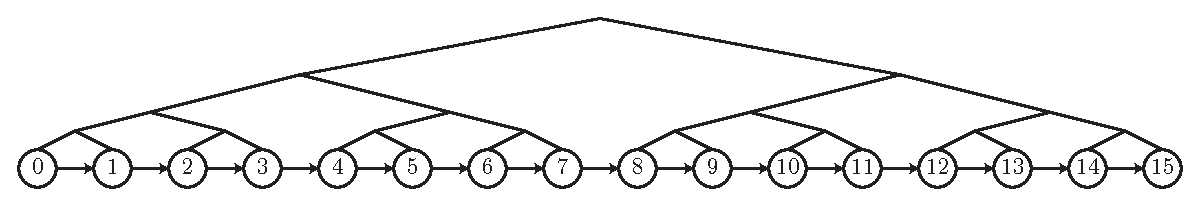
\includegraphics[width=16cm]{illustrations/nuts_tree.pdf}
\caption{A binary tree that results from running NUTS for 5 iterations. It has $2^5 = 16$ leafs. The leafs are connected by arrows to indicate that the path along the leafs is a valid leapfrog trajectory: the $i$th leaf ($i \in \{0 \ldots 15\}$) is the result of running the leapfrog algorithm for $i$ steps from leaf $0$.}
\label{fig_nuts_tree}
\end{figure}

In each iteration of NUTS, in addition to growing the tree, we check for U-turns. More specifically, we check the U-turn condition for the leftmost and rightmost leafs of all balanced subtrees. Fig. \ref{fig_nuts_uturn_leafs} illustrates each pair of leafs that need to be checked (in tree of height $5$) by a colored line. When checking for a U-turn, we check whether continuing the Hamiltonian dynamics in \textit{either} direction would result in the distance between the leafs to decrease. When checking the pair of leafs $(\theta_\text{left}, v_\text{left})$ and $(\theta_\text{right}, v_\text{right})$, this is derived in Eq. \ref{eq_uturn_both_dirs}.

\begin{figure}[ht]
\centering
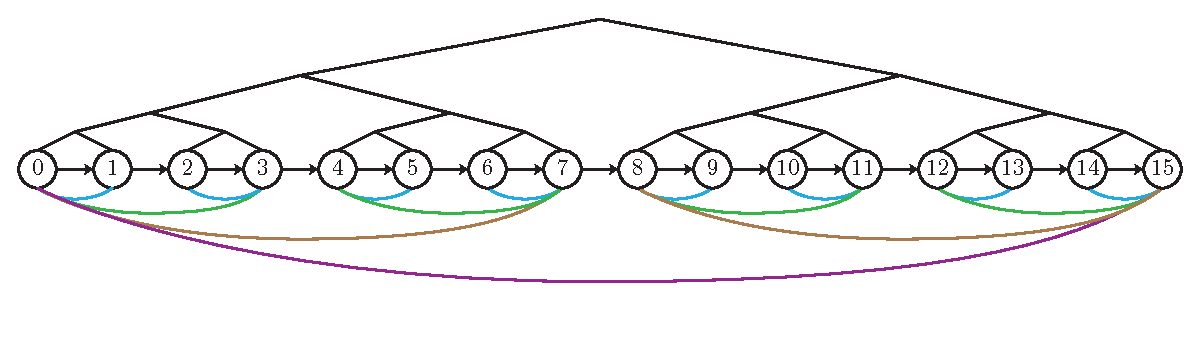
\includegraphics[width=16cm]{illustrations/nuts_uturn_leafs.pdf}
\caption{A binary tree that results from running NUTS for 5 iterations. Colored  lines connect each pair of leafs that need to be checked for a U-turn in a tree of height $5$.}
\label{fig_nuts_uturn_leafs}
\end{figure}

\begin{equation}
(\theta_\text{right} - \theta_\text{left}) \cdot v_\text{left} < 0
\quad \text{or} \quad
(\theta_\text{right} - \theta_\text{left}) \cdot v_\text{right} < 0
\label{eq_uturn_both_dirs}
\end{equation}

In order to preseve detailed balance, once we detect a U-turn (or a different termination criterion is reached, as discussed later), the tree stops growing and NUTS proposes a new state sampled from all \textit{candidate states} $\mathcal{C}$ along the leapfrog trajectory. The set of candidates states is a subset of all leafs in the tree $\mathcal{B}$. There is a deterministic process for mapping the set of all leafs to the set of candidate states $\mathcal{B} \rightarrow \mathcal{C}$. In Fig. \ref{fig_nuts_uturn_detailed_balance}, for example, if the initial state was $(\theta, v)$ and the particle leapfrogged until it reached $(\theta', v')$, the part of the trajectory between the cross and $(\theta', v')$ would not be considered part of valid samples $\mathcal{C}$. The reason is that if a particle started at $(\theta', v')$ and traveled toward $(\theta, v)$, it would \textit{always} stop at the cross, hence it would \textit{never} reach $(\theta, v)$. This scenario would break detailed balance, hence it must avoided. Recall that NUTS checks for a U-turn between the leftmost and rightmost leafs of all balanced subtrees each time the full tree doubles. If the U-turn is detected between the leftmost and rightmost leafs of the full tree, then any state along the leapfrog trajectory may be proposed without breaking detailed balance. However, if a U-turn is detected between anywhere \textit{within} the leafs that were just added to the full tree, \textit{only} those leafs may be proposed that existed \textit{before} the tree doubling.

While in HMC the mapping $(\theta, v) \rightarrow (\theta', v')$ is deterministic, in NUTS, it is random. Still, in both cases $Q(\theta', v'|\theta, v) = Q(\theta, v|\theta', v')$. In NUTS, this is achieved by sampling $(\theta', v')$ uniformly from $\mathcal{C}$ and designing $p(\mathcal{B}, \mathcal{C} \mid \theta, v, u)$ such that if $(\theta, r) \in \mathcal{C}$ and $\left(\theta^{\prime}, r^{\prime}\right) \in \mathcal{C}$, then for any $\mathcal{B}$, $p(\mathcal{B}, \mathcal{C} \mid \theta, v)=p(\mathcal{B}, \mathcal{C} \mid \theta', v')$. In other words, any two states in $\mathcal{C}$ have the same probability of generating the full tree $\mathcal{B}$, and $(\theta', v')$ is sampled uniformly from $\mathcal{C}$ .

Even though NUTS is closely related to HMC, it does not use Metropolis-Hastings sampling. Instead, it uses \textit{slice sampling} \cite{slice_sampling}. Slice sampling is motivated by the observation that in order to draw samples from a distribution, we can take uniform samples from the area under the curve of its density function. This is achieved by alternately sampling vertically and horizontally from this area, as illustrated in Fig. \ref{fig_slice_sampling}. When sampling horizontally, we map $(\theta, v) \rightarrow (\theta', v')$. In order to sample vertically, we define a \textit{slice variable} $u$​, which is a scalar variable representing the height. The joint distribution of $(\theta, v, u)$ is uniform under the curve $\pi(\theta, v)$:

\begin{equation}
p(\theta, v, u) \propto \mathbb{I}\left(u \in\left[0, \pi(\theta, v) \right]\right)
\end{equation}

When sampling vertically under the curve, we need to draw samples of the slice variable $u$ conditional on $(\theta, v)$. Since the joint distribution $(\theta, v, u)$ is distributed uniformly under $\pi(\theta, v)$, $u|(\theta, v)$ is also distributed uniformly under $\pi(\theta, v)$: $u|(\theta, v) \sim \text{Uniform}[0, \pi(\theta, v)]$. Similarly, in order to sample horizontally under the curve, we draw samples of $(\theta, v)$ conditional on the slice variable $u$. $(\theta, v)|u$ is distributed uniformly along the region where the slice variable falls under the curve: $(\theta, v) | u \sim \text{Uniform}\{(\theta, v), \pi(\theta, v) \geq u\}$. However, to improve numerical stability, is is better to work with $\log u$ instead of $u$. The distribution of $\log u$ is derived in Eq. \ref{eq_logu_distr}.

\begin{figure}[ht]
\centering
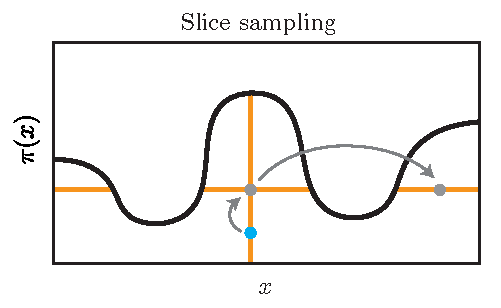
\includegraphics[width=7cm]{illustrations/slice_sampling.pdf}
\caption{During slice sampling, we alternately sample vertically and horizontally from the are under the target density function. For example, starting at the blue point, we would sample vertically along the vertical orange line and arrive at the first grey point. Then we would sample horizontally along the horizontal orange line, arriving the second grey point. This alternating cycle repeats indefinitely.}
\label{fig_slice_sampling}
\end{figure}


\begin{align}
\begin{split}
u &\sim \text{Unif}[0, \pi(\theta, v)] \\
\text{let} \ x &:= u/\pi(\theta, v) \Rightarrow x \sim \text{Unif}[0, 1], \  -\log(x) \sim \text{Exp}(1) \\
\log(u) &= \log(\pi(\theta, v) \times x) = \log\pi(\theta, v) - (-\log(x)) \\
\log(u) &\sim \log \pi(\theta, v) - \text{Exp}(1)
\end{split}
\label{eq_logu_distr}
\end{align}


Technically, in NUTS, we don't sample $(\theta,v,u)$ directly. Instead, we performs \textit{Gibbs sampling} over the joint distribution $(\theta, v, u, \mathcal{B}, \mathcal{C})$. Gibbs sampling simply means that we iteratively sample each variable from its \textit{full-conditional} distribution, i.e. its distribution conditional on all the other variables. This is performed as described in Algorithm \ref{alg_nuts_gibbs}. All of the steps are valid Gibbs updates because they resample each variable (or set of variables) from their full-conditional distribution. In step 3, we first build the leapfrog trajectory $\mathcal{B}$. Then, when mapping $\mathcal{B} \rightarrow \mathcal{C}$, we only consider those states $(\theta', v')$ that satisfy detailed balance \textit{and} constitute a valid update under slice sampling, i.e. only those where $u \leq \pi(\theta', v')$.

\begin{algorithm}
\caption{NUTS as Gibbs sampling over $(\theta, v, u, \mathcal{B}, \mathcal{C})$}
\label{alg_nuts_gibbs}
\begin{algorithmic}
\For{$\textrm{step} \gets 1 \ldots n_\textrm{samples}$} 
\State resample $v \sim \mathcal{N}(0, \sigma^2)$
\State resample $u \sim \text{Uniform} [0, \pi(\theta, v)]$
\State resample $\mathcal{B}, \mathcal{C} \sim p(\mathcal{B}, \mathcal{C} \mid \theta, v, u)$
\State resample $\theta, v \sim \text{Uniform}[\mathcal{C}]$
\EndFor
\end{algorithmic}
\end{algorithm}

Also, in addition to U-turns, we add two additional stopping criteria. First, we define a maximum tree depth, which is equivalent to defining the maximum number of leapfrog steps. This is to ensure that the program terminates even in absence of U-turns and we don't run out of memory. Second, we define a maximum leapfrog error $\Delta_\text{max}$. However, imposing a maximum error \textit{does} violate detailed balance. Hence $\Delta_\text{max}$ needs to be made very large, such that it is only reached if the simulation is poorly setup, i.e. by setting the step size too large.

\subsubsection{Iterative NUTs}

In the original NUTS algorithm, the process for building a tree, including all stopping conditions, is recursive. However, it is difficult to implement a recursive algorithm efficiently. The developers behind NumPyro (a probabilistic programming library) solved this problem by developing \textit{Iterative NUTS}, which is an iterative formulation of NUTS, meaning it can be implemented much more efficiently \cite{numpyro}.

The process of building a tree is described through a nested for loop. The outer loop iterates through tree height, $h \in \{1, 2, 4, 8, 16 \ldots \}$. Each height $h$ corresponds to $2^h$ leafs (leapfrog steps). The inner loop iterates though each leaf, first generating it using the leapfrog algorithm, then checking for a U-turn. The outer loop is responsible for setting a forwards / backwards direction and checking whether any stopping condition was reached within the inner loop.

The main challenge in formulating NUTS as an iterative algorithm is to find an efficient way of checking U-turns. For example, imagine that we want to check for U-turns in a tree of height 5, as illustrated in Fig. \ref{fig_iterative_nuts_indexing}. First, notice in the figure that each pair of leafs that we check for a U-turn consists of one leaf with an odd index and one leaf with an even index. This means that as we iterate through the leafs, we can use even nodes to store temporary state and odd nodes to check for U-turns agains these previously-generated states. For example, at leaf 0, we would store its value and at leaf 1, we would check for a U-turn between leaf 0 and leaf 1. Notice that we do not need to store the value of leaf 1 because leaf 1 is not compared to any leaf with index greater than 1.

\begin{figure}[ht]
\centering
\makebox[\textwidth][c]{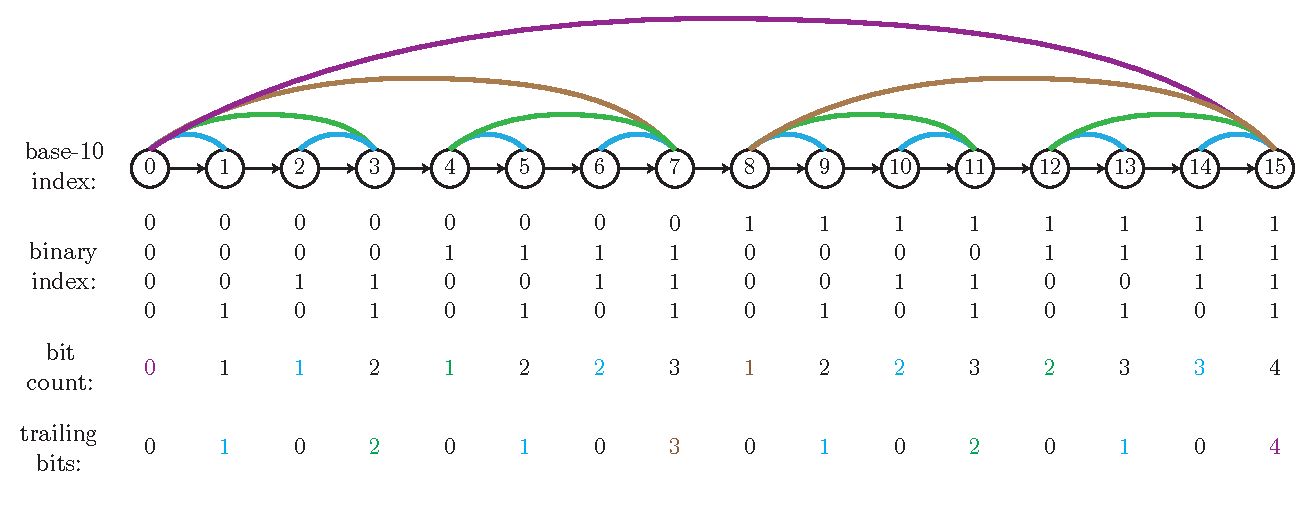
\includegraphics[width=17cm]{illustrations/iterative_nuts_indexing.pdf}}
\caption{The 16 nodes correspond to the leafs of a height-5 tree. Colored lines indicate which pairs of leafs need to be checked for a U-turn. Each leaf is indexed in base 10 and base 2. The last two rows show the bit count and number of trailing bits of the binary representation of each index.}
\label{fig_iterative_nuts_indexing}
\end{figure}

Since NUTS is based on a balanced binary tree, it is natural to index each leaf of the tree using binary numbers -- the binary index of each leaf corresponds closely to the position of the leaf within the tree. For example, observe that the number of trailing bits of each even leaf dictates how many past leafs we need to check for a U-turn. For instance, the leaf 1 has binary representation 01, hence its number of trailing bits is 1. This is because it is the rightmost leaf only within a subtree of height 1. On the other hand, the leaf 7 has binary representation 111 and 3 trailing bits, because is the rightmost leaf in subtrees of height 1, 2, and 3. Hence, it must be compared to 3 other leafs when checking for U-turns.

Also, observe that we do not need to store the value of each even leaf. Instead, for a tree of height $h$, we can get away with storing just $\log_2 h$ leafs. We can use the bit count of each even leaf to decide where in this array it should be stores. We will store leaf 0 in the 0th element of the array. We must keep this leaf indefinitely and no other leaf has bitcount 0, so this value will never get overwritten. We will store each leaf with bitcount 1 in the first element of the array. There are multiple leafs with bitcount 1, so the first element of the array will get overwritten multiple times, but each time this happens, we no longer need to keep the previous values. In general, we will store \textit{each} odd leaf as the $\text{bitcount}(i)$-th element in the array.

Putting all this together, the following algorithm is a valid pseudocode implementation of \textit{Iterative NUTS}:

\newgeometry{margin=1.5cm}
\begin{algorithm}
\small
\caption{Iterative NUTS}
\label{alg_nuts}
\begin{algorithmic}
\For{$\textrm{step} \gets 1 \ldots n_\textrm{samples}$} \Comment{generate $n_\textrm{samples}$ from target distribution}
	\State $\theta^+, \theta^-, \theta_\textrm{out} \gets \theta $ \Comment{initialize leftmost ($-$) and rightmost ($+$) leaf}
	\State $v^+, v^-, v_\textrm{out} \gets v $
	\State $n_\textrm{valid leafs} \gets 1$ \Comment{size of $\mathcal{C}$}
	\State resample $\log u \sim \log \pi(\theta, v) - \textrm{Exp}(1)$ \Comment{resample log of slice variable}
	
	\State $\textrm{stop} \gets \textrm{False}$ \Comment{becomes true if any termination condition is reached}
	\State resample $v \sim N(0, \sigma^2)$ \Comment{resample momentum}
	\For{$i \gets 1 \ldots 2^\textrm{MaxTreeHeight}$} \Comment{loop through leafs}
		
		% tree has doubled
		\If{$\textrm{IsPowerOfTwo}(i)$} \Comment{tree is about to double}
			\State $\theta_\textrm{out}, v_\textrm{out} \gets \theta_\textrm{subtree out}, v_\textrm{subtree out}$ \Comment{leafs are in $\mathcal{C}$ only if there were no U-turns}
			\State resample $\textrm{direction}_\textrm{new} \sim \textrm{Uniform}[\{-1, 1\}]$ \Comment{decide whether to leapfrog forwards or backwards}
			\If{$\textrm{direction}_\textrm{new} \ne \textrm{direction}$} \Comment{when direction changes, flip the tree}
				\State $\theta^+, \theta^- \gets \theta^-, \theta^+$
				\State $v^+, v^- \gets v^-, v^+$
			\EndIf
			\State $\textrm{direction} \gets \textrm{direction}_\textrm{new}$
			\State $\textrm{checkpoints}[0] \gets (\theta^-, v^-)$ \Comment{checkpoint leftmost leaf}
		\EndIf
		
		% leapfrog
		\State $\theta^+, v^+ \gets \textrm{Leapfrog}(\theta^+, v^+, \textrm{direction})$ \Comment{leapfrog a single step (forwards or backwards in time)}
		
		% update chekpoints
		\If{$i$ is even} \Comment{update checkpoints}
			\State $\textrm{checkpoints}[\textrm{BitCount}(i)] \gets (\theta, v)$
		
		% check u-turns
		\ElsIf{$i$ is odd} \Comment{check U-turns}
			\For{$j \gets \textrm{BitCount}(i)-\textrm{NumTrailingBits}(i) \ldots \textrm{NumTrailingBits}(i)$}
				\State $\theta^*, v^* \gets \textrm{checkpoints}[j]$
				\State $\textrm{stop} \gets \textrm{stop} \ \textrm{or} \ (\theta^+ - \theta^*) \cdot v^* < 0 \ \textrm{or} \ (\theta^+ - \theta^*) \cdot v^+ < 0$
		    \EndFor
		\EndIf
		
		% check max error
		\State $\textrm{stop} \gets \textrm{stop} \ \textrm{or} \ \Delta_\mathrm{max} < \log u - \log \pi(\theta^+, v^+)$ \Comment{check maximum leapfrog error}
			
		% update output
		\If{stop}
			\State $\theta, v \gets \theta_\textrm{out}, v_\textrm{out}$ \Comment{$\theta_\textrm{out}, v_\textrm{out}$ were sampled uniformly from the valid leafs}
			\State break
		\Else
			\If{$\log u \leq \log \pi(\theta^+, v^+)$} \Comment{slice sampling}
				\State with prob. $1/n_\textrm{valid leafs}$, set $\theta_\textrm{subtree out}, v_\textrm{subtree out} \gets \theta^+, v^+$ \Comment{resample output leaf}
				\State $n_\textrm{valid leafs} \gets n_\textrm{valid leafs} + 1$
			\EndIf
		\EndIf
		
	\EndFor
\EndFor
\end{algorithmic}
\end{algorithm}
\restoregeometry

\section{Implementation}

One of the strongest limitations of MCMC-based Bayesian neural networks (compared to standard neural networks) is that they are orders of magnitude computationally more expensive to train and run inference on. For this reason, it is essential that any implementation of a BNN is as computationally-efficient as possible. The implementation behind this project utilizes several related tricks to achieve this (JAX, JIT, TPUs, SPMD), which are described below.

All mathematical operations are implemented in JAX, an open-source machine learning library developed by Google. This includes the neural network, gradient-descent training, and 

\section{Results}
\label{sec_results}

\begin{figure}[ht]
\centering
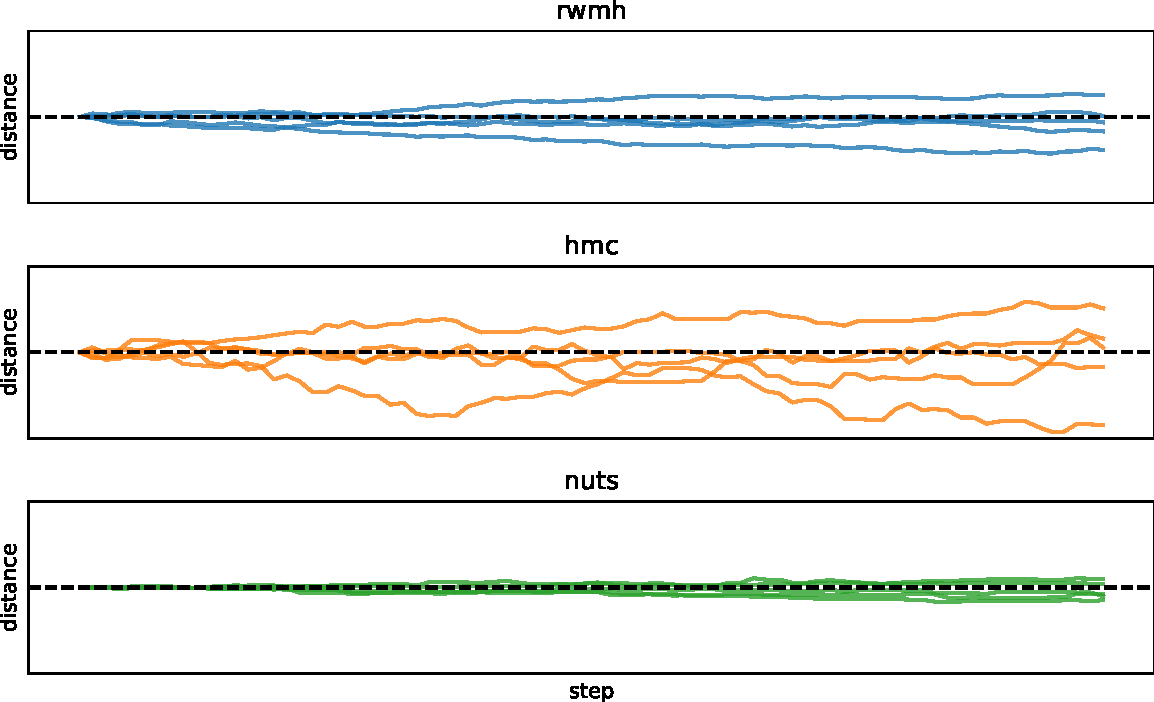
\includegraphics[width=16cm]{plots/uci_param_history.pdf}
\caption{}
\label{fig_uci_param_history}
\end{figure}

\begin{figure}[ht]
\centering
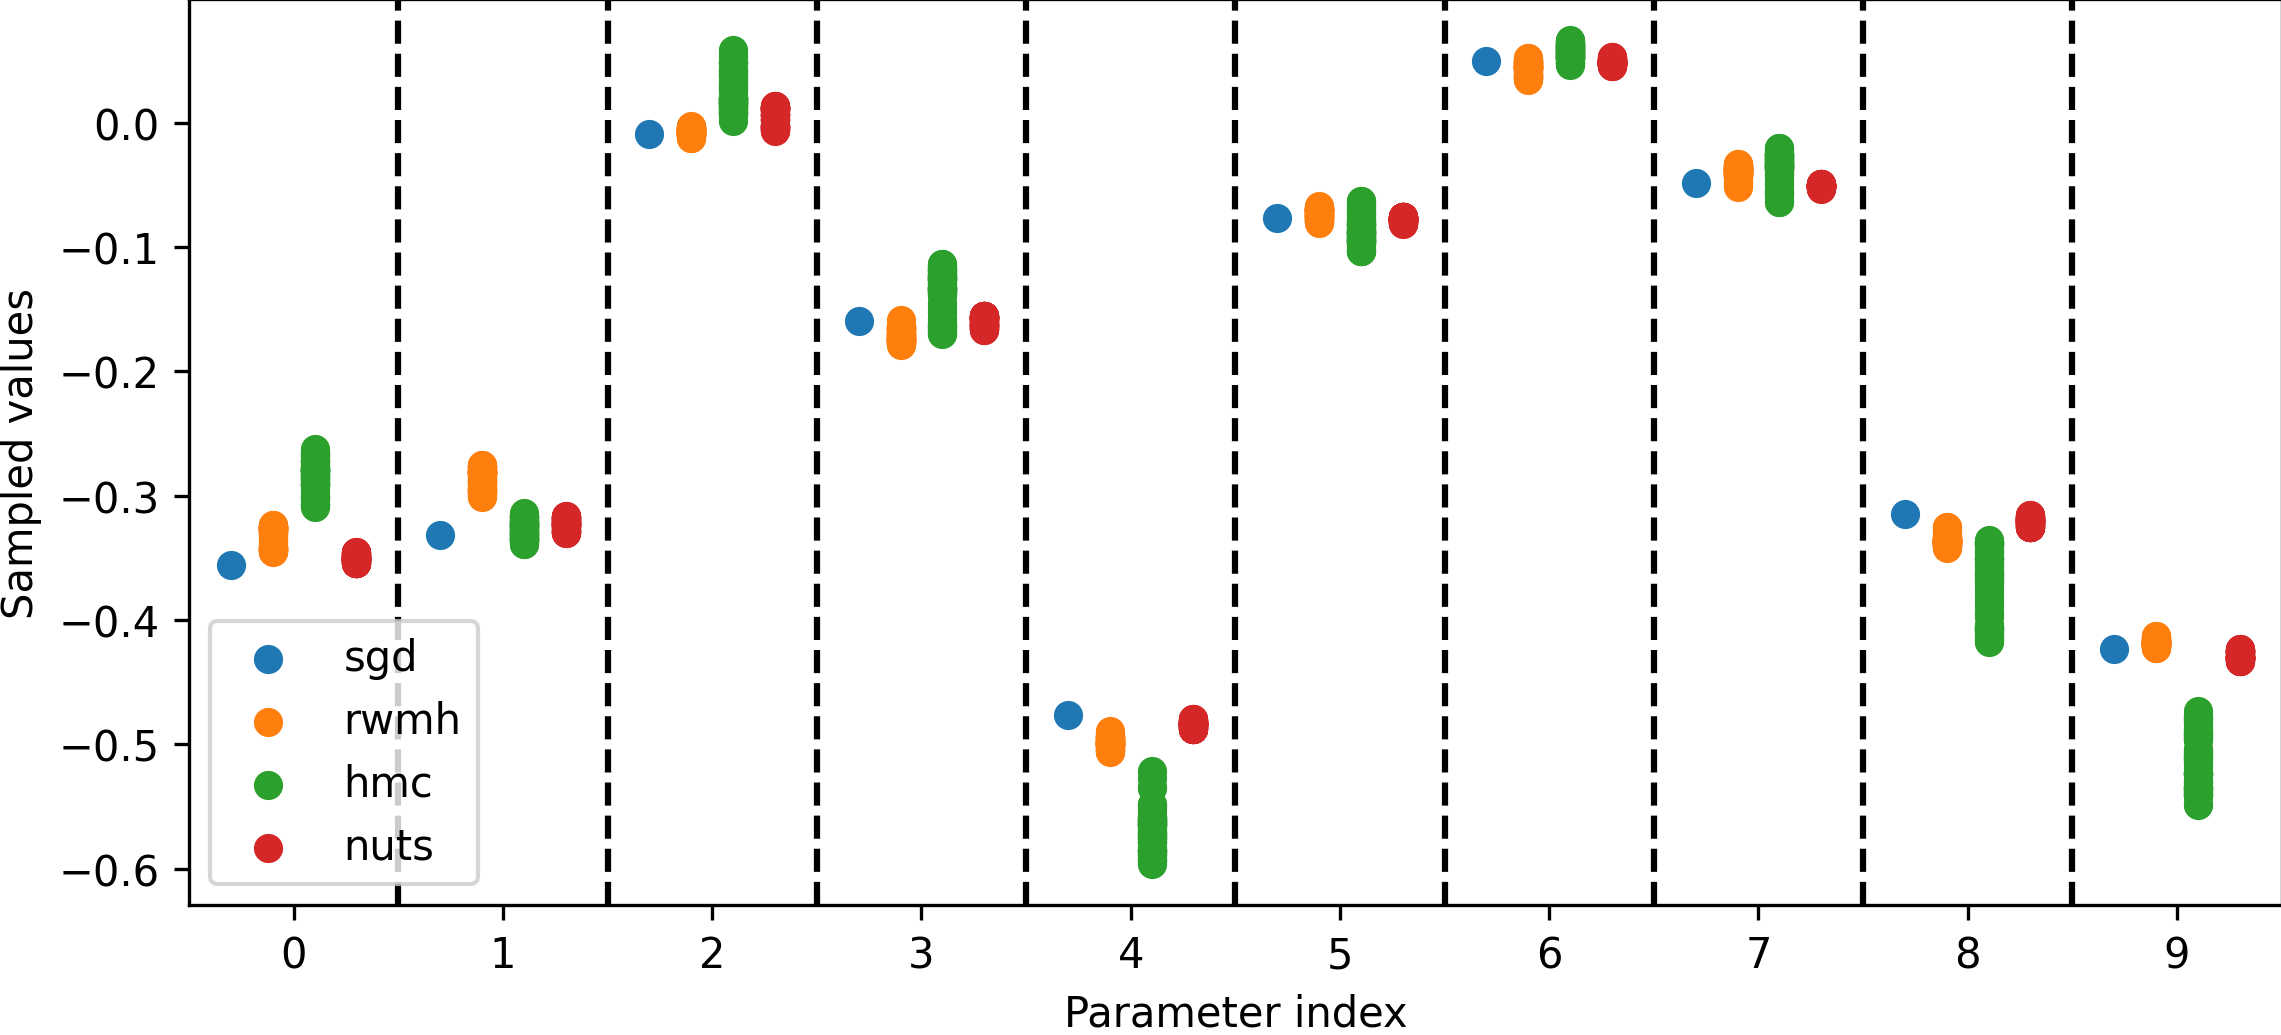
\includegraphics[width=15cm]{plots/uci_param_distribution.png}
\caption{}
\label{fig_uci_param_distribution}
\end{figure}

\begin{figure}[ht]
\centering
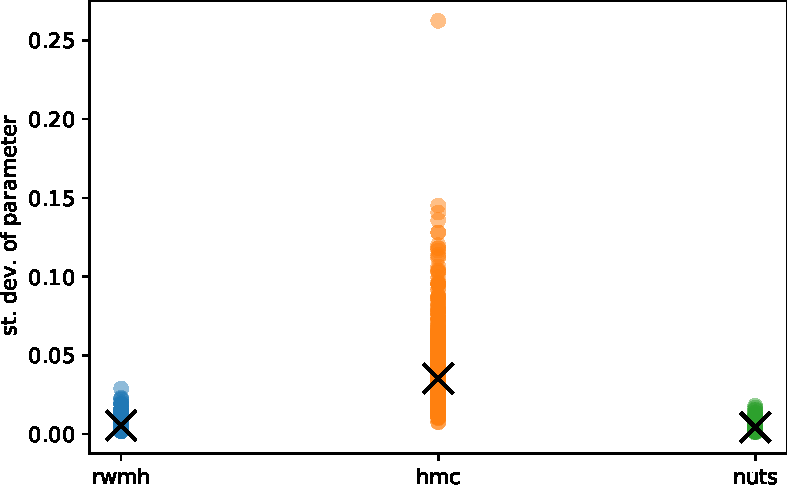
\includegraphics[width=10cm]{plots/uci_param_stdev.pdf}
\caption{}
\label{fig_uci_param_stdev}
\end{figure}

\begin{figure}[ht]
\centering
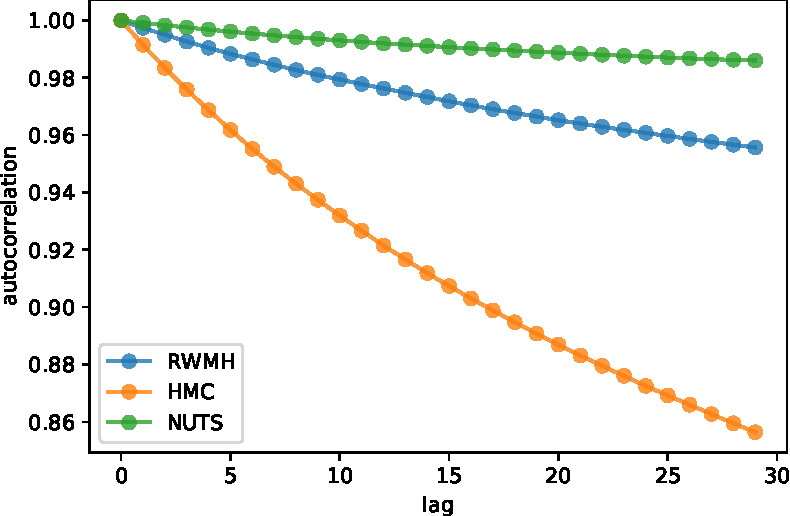
\includegraphics[width=10cm]{plots/uci_param_autocor.pdf}
\caption{}
\label{fig_uci_param_autocor}
\end{figure}

\begin{figure}[ht]
\centering
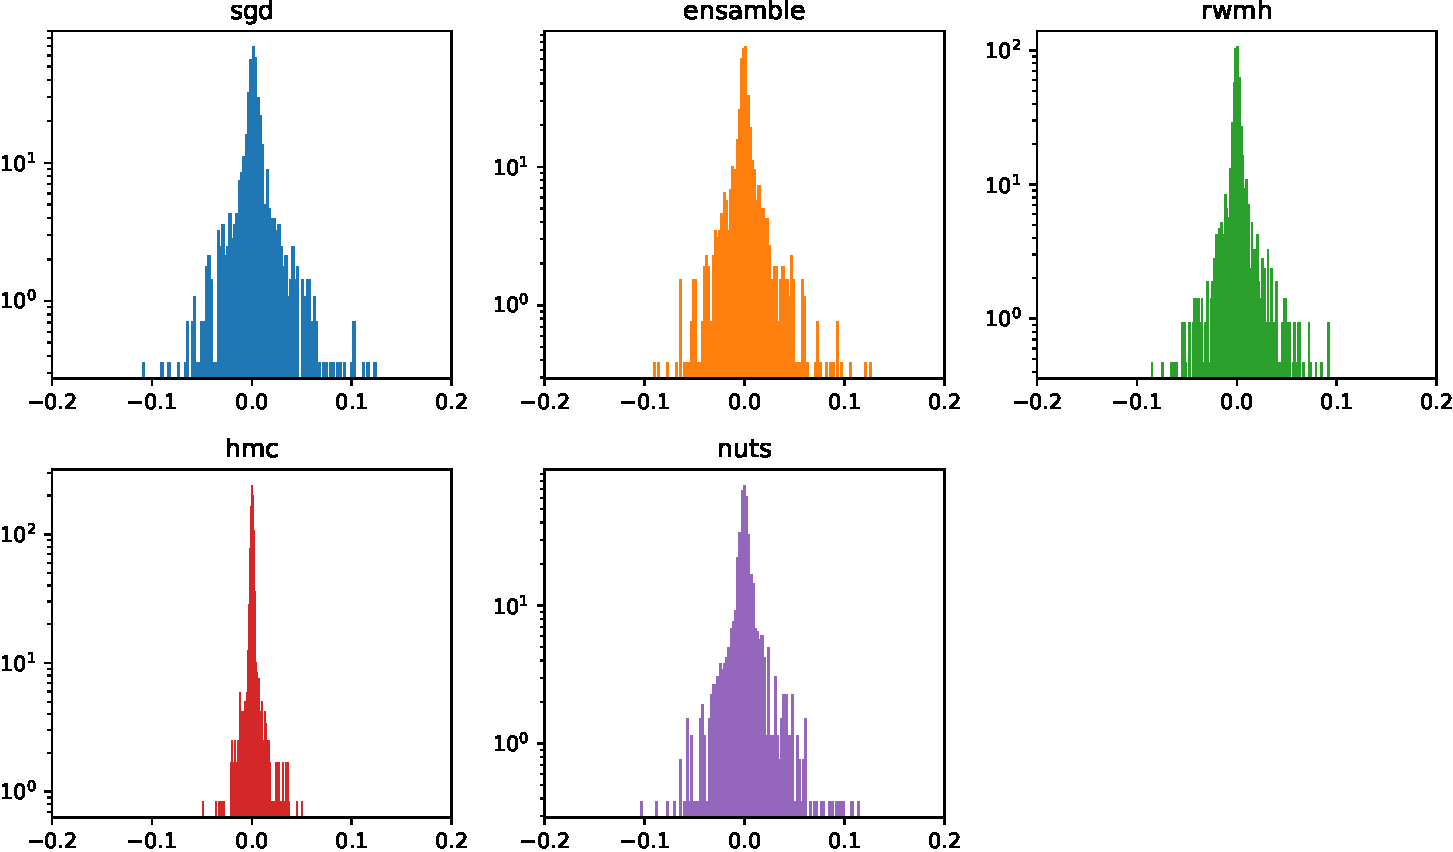
\includegraphics[width=15cm]{plots/uci_residuals_hist.pdf}
\caption{}
\label{fig_uci_residuals_hist}
\end{figure}

% TODO: table: MSE
% TODO: table: log-likelihood

\begin{figure}[ht]
\centering
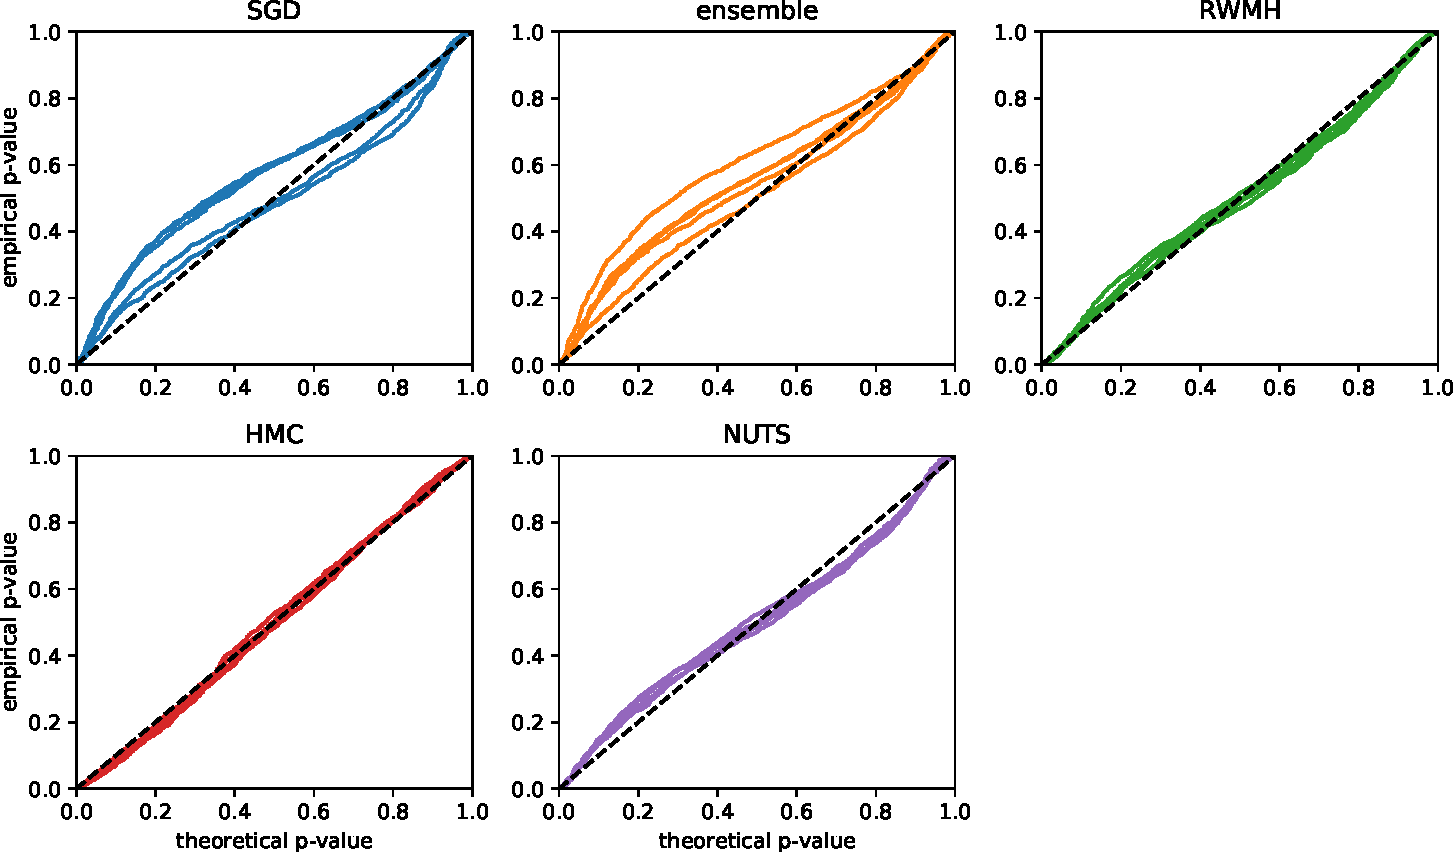
\includegraphics[width=15cm]{plots/uci_residuals_pvals.pdf}
\caption{}
\label{fig_uci_residuals_pvals}
\end{figure}

\section{Conclusion}


\bibliographystyle{plain}
\bibliography{references.bib}
\end{document}
